\chapter{The RISC-V processor}\label{Chapter:5}
    We are finally at a point where we can start building the RISC-V CPU in SME. At the start of this project I followed the approach described in chapter 4 of the RISC-V book \cite{riscVbook}, but when a functioning CPU was made I quickly came to the realization that the version described in the book was quite inadequate. It only supported a handful instructions, which is not enough to run any but the simplest of programs. 
    
    Therefore I had to sit down and design a version with the requirement of supporting all 49 basic RISC-V instructions \texttt{RV64I}. This design of course took foundation in the book version, with improvements from the lessons learned from the first implementation.
    
    Throughout this chapter we will go through the new design, which can be found here\footnote{\url{https://github.com/DanielRamyar/Master_Thesis/tree/master/SME_Implementations/SingleCycleRISCV2}}.

\section{Single Cycle RISC-V Units}\label{section:riscunits}
    In this section we will explain the function of each of the 12 unique units, used in the implementation of the CPU. This design is single cycle, meaning that only one instruction is executed per clock cycle. 

    \subsection{Program Counter}
        The \textit{program counter}, PC for short, keeps track of where in the program we are located and is a fairly simple unit. It can we thought of as a single register, which holds the address of the current instruction.
        
        To implement the PC unit we create a clocked SME process. It needs to be clocked, meaning the unit will activate on a rising clock edge, as it will part of a closed loop circuit, when we later connect the units. If no unit is clocked in a closed loop, there is no way of knowing, where to begin sending signals. Therefore the PC was chosen to be clocked, as it seemed like the most logical place to start the signal propagation.
        
        The PC process contains a single \texttt{ulong} integer, which will hold the instruction address. The input bus contains the address of the next instruction and the output bus the current. You may ask how the process outputs the current address, when it reads the next address first. Remember that the process is clocked, so when it reads the next address input, it will actually contain the address calculated in the previous clock cycle, as the bus hasn't been updated yet. This would then be the correct address in the current clock cycle.
        
        The PC process has been illustrated in Figure \ref{fig:PC} and a code segment is shown in Listing \ref{PCSME}. 
        
        
        
        \begin{figure}[h!]
            \centering
            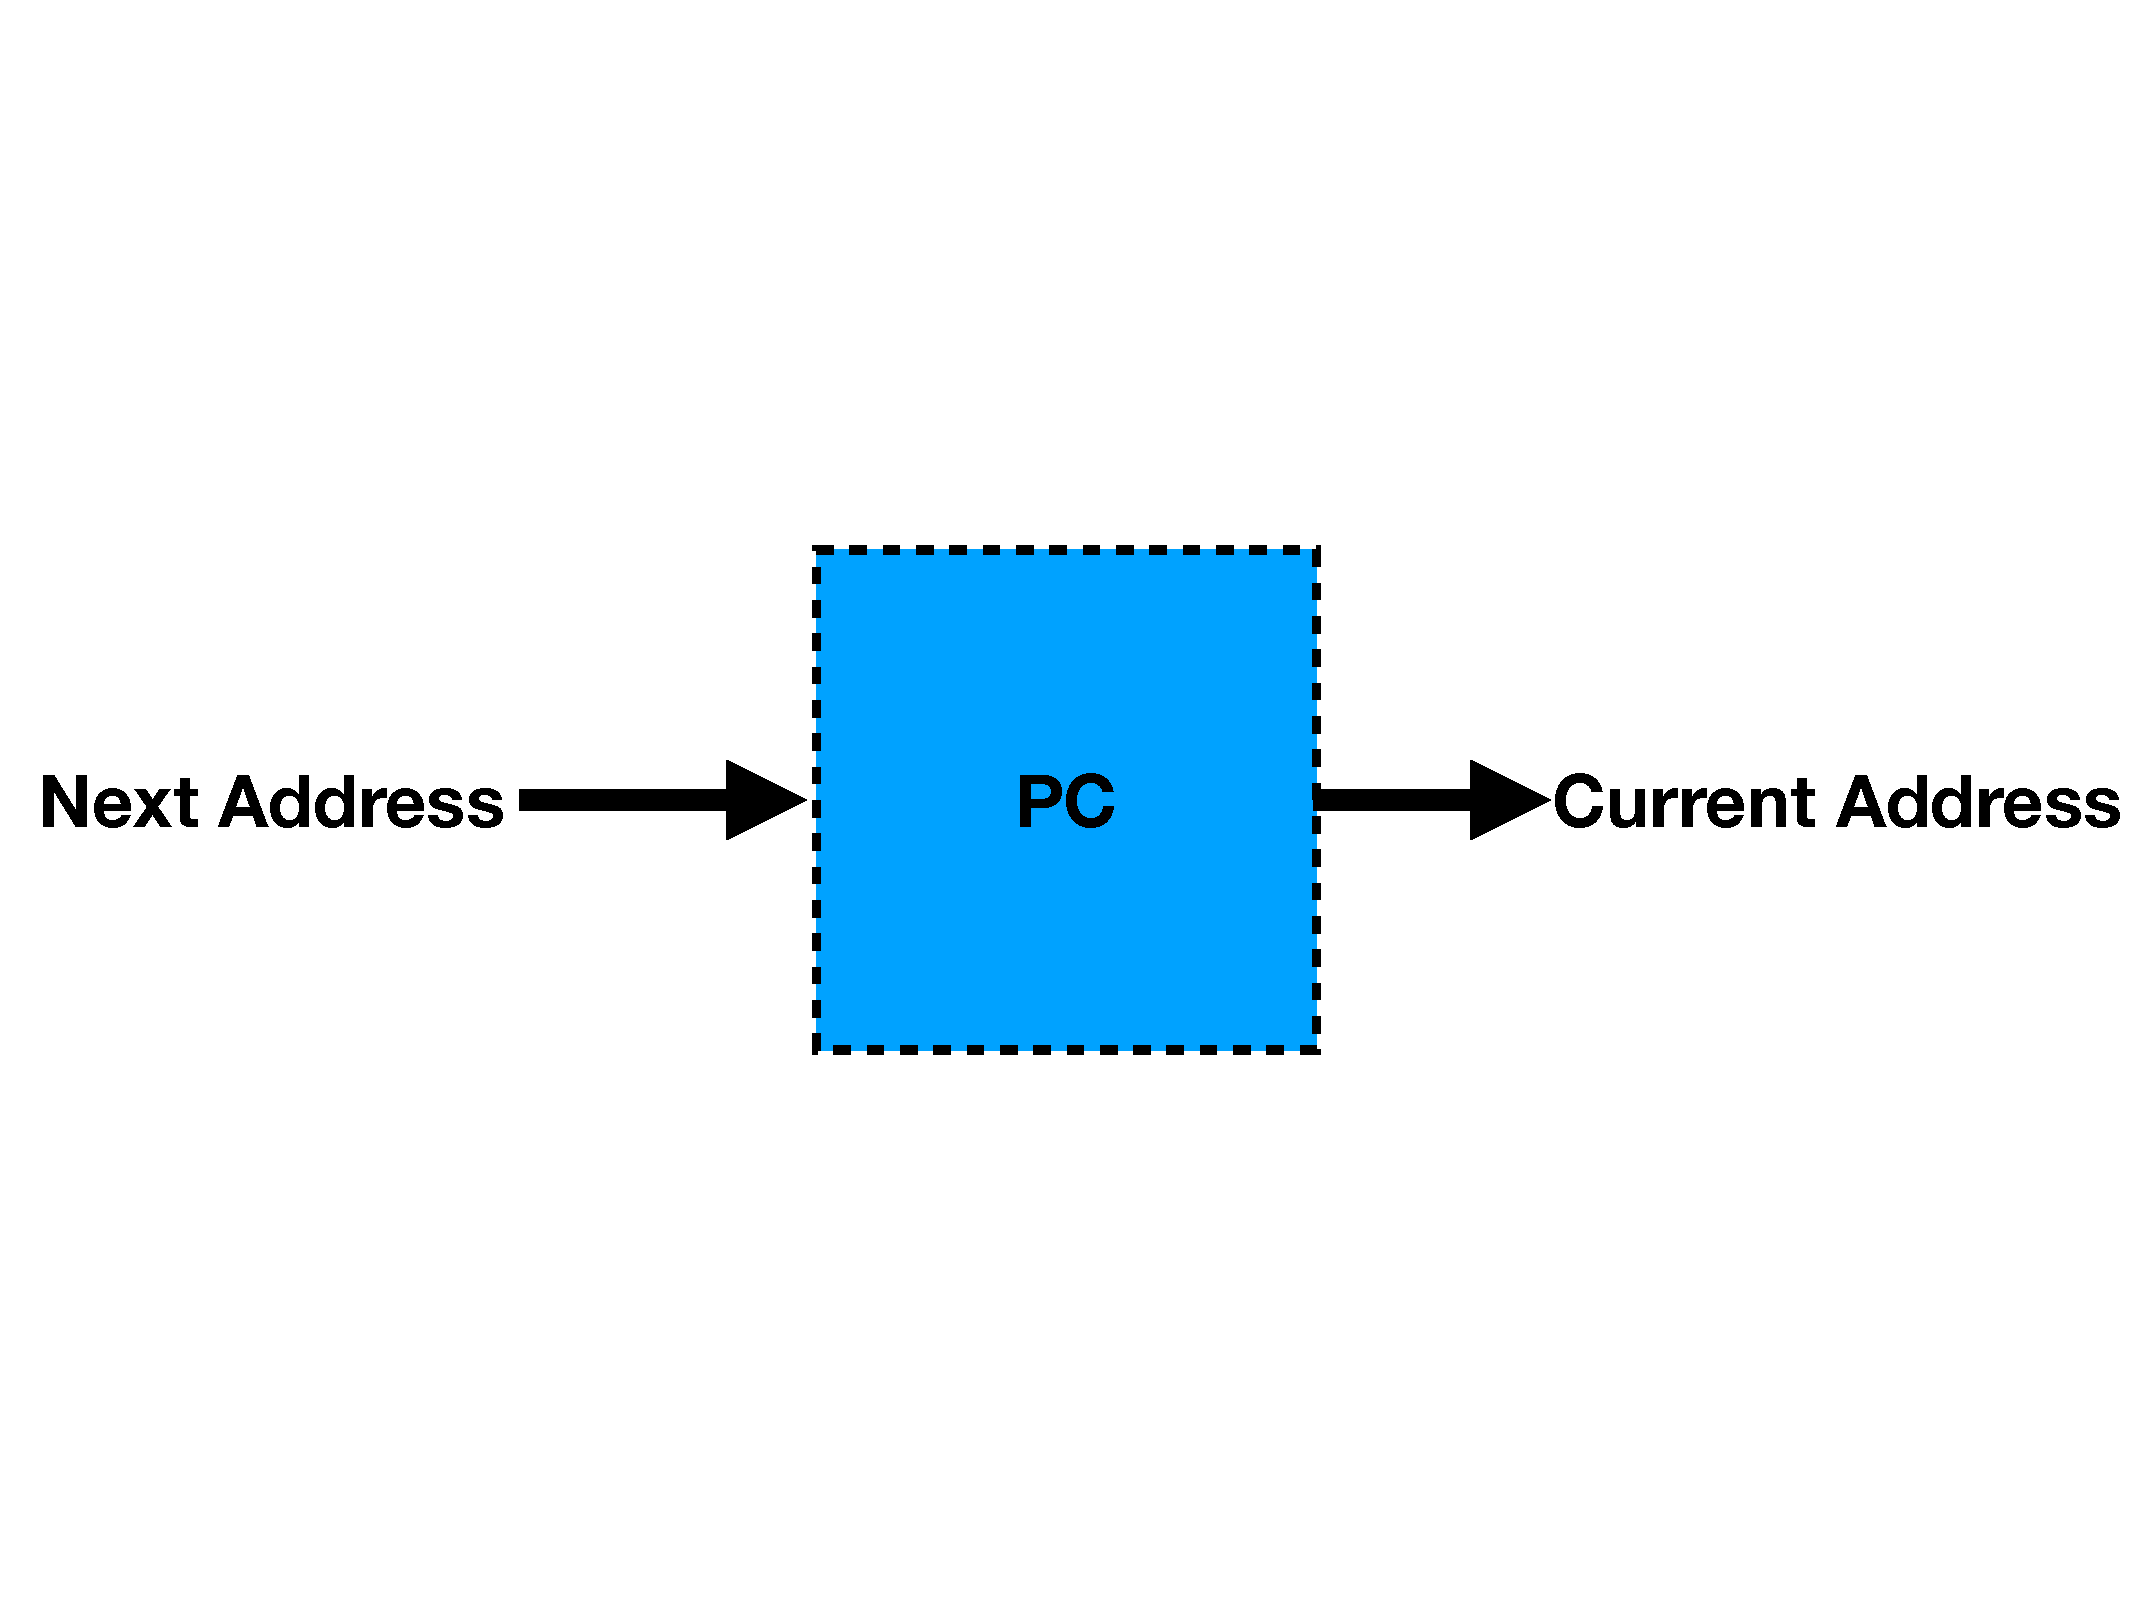
\includegraphics[scale=0.2]{pictures/PC.pdf}
            \caption{Illustration of the clocked \texttt{program counter} process having the next address as input and current address as output. The dashed square indicates a clocked process.}
            \label{fig:PC}
        \end{figure}
    
        \begin{minipage}{\linewidth}
            \begin{lstlisting}[language={[Sharp]C}, caption={A slice of the PC unit SME code, which contains variable that holds the input address. On every cycle edge it then holds and outputs the current address.},captionpos=b, label = PCSME]
...
    ulong address_hold;

    protected override void OnTick() {
        address_hold = m_Input.Address;
        Output.Address = address_hold;
    }
            \end{lstlisting}
        \end{minipage}   
    
    \subsection{Instruction Memory}
        The \textit{instruction memory}, IM for short, contains the program to be run on the CPU. To implement the instruction memory we create a SME process. It contains a byte array with the instructions to be run. A byte array was chosen to respect the conventions discussed in \ref{section:datatranserinstructions}. This also has the added benefit of having a built-in C$\scalerel*{\#}{X}$ function to read a binary file, which automatically puts the instructions contained within the file, in the correct array format. 
        
        The instructions can also be hand written when declaring the array. Since an instruction is 32-bits, 4 elements in the array are needed to form an instruction, where index 0-3 contains the first instruction.
        
        The instruction memory process has a single input from the program counter, which it uses access the correct instructions. In each cycle we first check whether the address given lies within the instruction array range, if not we shut down the CPU.
        We then construct an instruction, using methods discussed in \ref{section:Operators}, to a temporary variable.
        
        The register fields are then sliced out of this variable and put in the corresponding output buses, \texttt{Read RS1, RS2} and \texttt{Write RS}. The full instruction is also outputted to its own bus, \texttt{Instruction}. Lastly we tell the simulation process to keep the CPU running by asserting the \texttt{CPU} bus. The instruction memory process has been illustrated in Figure \ref{fig:IM} and a code segment is shown Listing \ref{IMSME} explaining parts of the code. 
     
        \begin{figure}[h!]
            \centering
            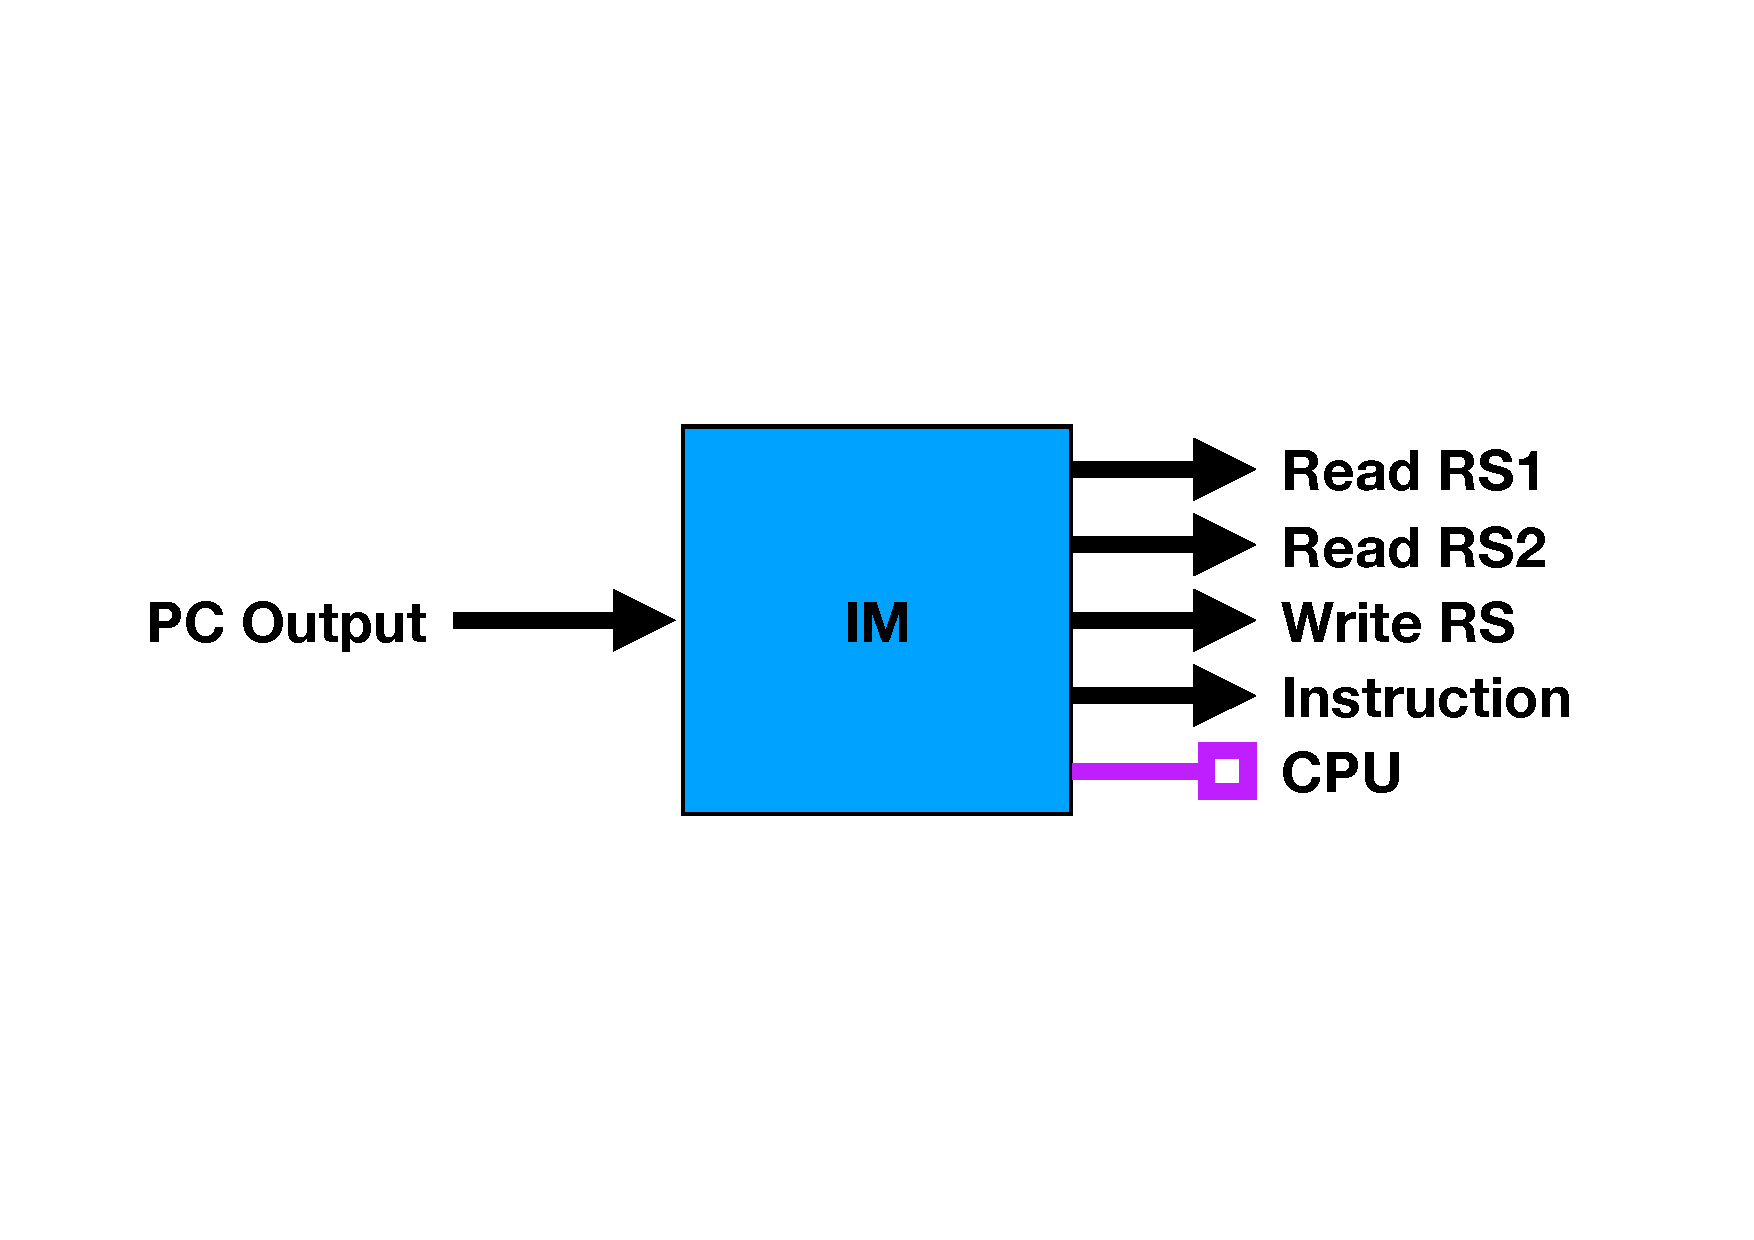
\includegraphics[scale=0.3]{pictures/IM.pdf}
            \caption{Illustration of the \texttt{instruction memory} process, taking the PC output as input and outputting to the 5 buses, \texttt{Read RS1 and RS2}, \texttt{Write RS}, \texttt{Instruction} and \texttt{CPU}.}
            \label{fig:IM}
        \end{figure}
    
        \begin{minipage}{\linewidth}
            \begin{lstlisting}[language={[Sharp]C}, caption={A slice of the Instruction Memory unit SME code. It contains a single byte array, which holds all the instructions to be run. First we check whether the given address to be accessed lies within instruction array, if not we shut down the CPU. We then use the address to access the correct array elements and create a temporary variable, which contains the instruction, as shown in lines 9-12. Hereafter we slice out the fields in the instruction and place the values in the correct busses. Lastly we tell the simulator to keep the CPU running using the CPU bus.},captionpos=b, label = IMSME]
...
    private readonly byte[] Instruction_Memory = System.IO.File.ReadAllBytes("/Users/danielramyar/Downloads/fibo.bin");
            
    protected override void OnTick() {
        ulong temp_address = m_input.Address;
        uint temp_instruction;
            
        if (temp_address >= 0 && temp_address < (uint)Instruction_Memory.Length) {
            temp_instruction = 0u | (uint)Instruction_Memory[temp_address]     << 24
                                  | (uint)Instruction_Memory[temp_address + 1] << 16
                                  | (uint)Instruction_Memory[temp_address + 2] << 8
                                  | (uint)Instruction_Memory[temp_address + 3];
            
            m_Instruction.Current = temp_instruction;
            m_read_1.Address = (uint)temp_instruction >> 15 & (uint)31; 
            m_read_2.Address = (uint)temp_instruction >> 20 & (uint)31; 
            m_write.Address  = (uint)temp_instruction >> 7  & (uint)31; 
            
            m_CPU.Running = true; // Keep CPU running
        }
        else {
            temp_instruction = 0u; // No Instruction
            ...  // Same as in the if statement
            m_CPU.Running = false; // Turn of cpu no more instructions
    }
            \end{lstlisting}
        \end{minipage}  
        
        
        
    
    \subsection{Next instruction Unit}
        To calculate the address of the next instruction in the queue I have created a unit called \texttt{Next}. This unit is very simple, as its only function is to increment the value found in the PC output bus by 4. We increment by 4, since each instruction is 32 bits long and since our instructions are contained in a byte array, we need to move 4 bytes every time we want to access the following instruction. For example if we are placed at index 0, we would have to go to index 4 to access the next instruction (index 0-3 contains instruction 1 and index 4-7 the next).
        
        The next instruction process has the the output from the program counter as input and sends the incremented address to the \texttt{Next Output} bus. The \texttt{Next} process is illustrated in \ref{fig:NEXT} and a code segment is shown in Listing \ref{NEXTSME}.
        
        \begin{figure}[h!]
            \centering
            \includegraphics[scale=0.34]{pictures/Next.pdf}
            \caption{Illustration of the \texttt{next} process, taking the \texttt{PC output} as input and outputs the next instruction address to the \texttt{next output} bus.}
            \label{fig:NEXT}
        \end{figure}
    
        \begin{minipage}{\linewidth}
            \begin{lstlisting}[language={[Sharp]C}, caption={A slice of the \texttt{Next} process SME code. Here we declare a temporary varible, which contains the program counter output. We increment the temporary variable by four and place it in the output bus.},captionpos=b, label = NEXTSME]
...
    ulong temp;
    
    protected override void OnTick() {
        temp = m_Input.Address + 4;
        Output.Address = temp;
    }
            \end{lstlisting}
        \end{minipage}  
        
    
    \subsection{Register}
        The \texttt{register}, or RS for short, is a small data storage location for operands of instructions among others (see Table \ref{table:RISCVRegister}). It can be accessed by specifying a register address in an instruction. 
        
        Since R-type instructions use two operands to execute an arithmetic operation, the register has two input lines carrying the address to the specified registers and two output lines carrying the data in the read registers.
        
        Furthermore the result needs to get stored, therefore we need two additional lines one carrying the result of an operation and the other an address for the storage location. To avoid any unintentional write backs to the register, we introduce a write control line, which is asserted if write back is intended.
        
        In SME the register is declared as a process containing a signed 64-bit array with 32 entries. To ensure the latest data is always read, we write to the register as the first thing. Since register 0 is hard-wired to zero according to the conventions, we make sure that the write back address lies within the range 1-31 and that the write control is asserted.
        Lastly we check if the read addresses lies within the range of the register and then output the data in the read registers to the corresponding buses. The \texttt{register} process is illustrated in Figure \ref{fig:REGISTER} and a code segment shown in Listing \ref{REGISTER}.
    
        \begin{figure}[h!]
            \centering
            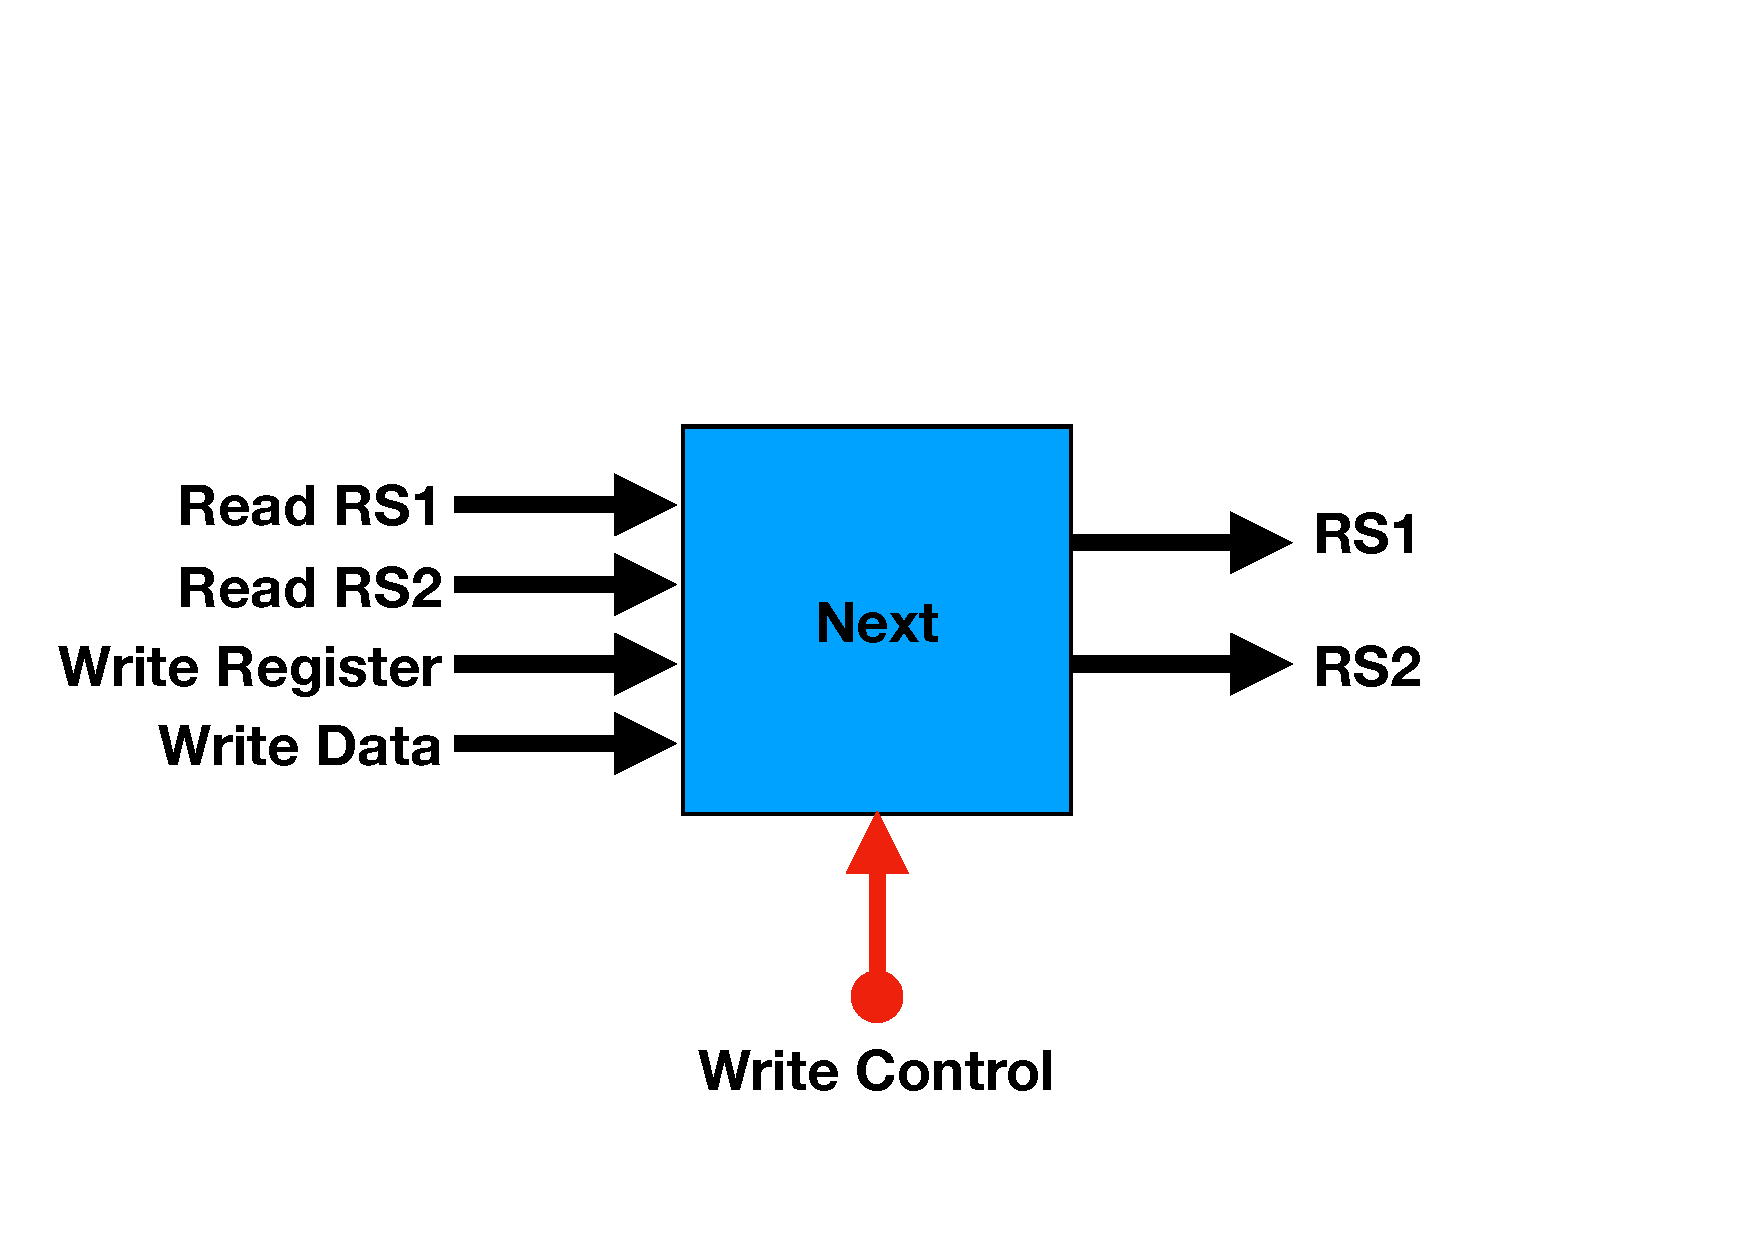
\includegraphics[scale=0.29]{pictures/REGISTER.pdf}
            \caption{Illustration of the \texttt{register} process. It gets its information on which register addresses to read from \texttt{Read RS1, RS2} buses. To write data the register uses \texttt{write register} bus to know which register to write to, the \texttt{write data} bus contains the data to be written and the \texttt{write control} bus authorize whether the register should write or not.}
            \label{fig:REGISTER}
        \end{figure}
    
        \begin{minipage}{\linewidth}
            \begin{lstlisting}[language={[Sharp]C}, caption={A slice of the \texttt{register} process SME code. The register is declared as a signed 64-bit array with 32 elements. In every clock cycle the process checks if the write control signal is asserted. If it is, we check if the address to be written lies within the register range and is above 0, as this register is reserved to be hard-wired zero. Lastly the process reads the two specified registers and if they lie within the register range, they get outputted to the corresponding buses.},captionpos=b, label = REGISTER]
...
    private readonly long[] m_register = {0, 0, 0, 0, 0, 0, 0, 0,
                                          0, 0, 0, 0, 0, 0, 0, 0,
                                          0, 0, 0, 0, 0, 0, 0, 0,
                                          0, 0, 0, 0, 0, 0, 0, 0,};
            
    protected override void OnTick() {
        if (m_write_control.Enable == true && m_write.Address > 0 && m_write.Address < 32) {
            m_register[m_write.Address] = m_write_data.Data;          
        }
        if (m_read_1.Address >= 0 && m_read_1.Address < 32) { 
            output_1.Data = m_register[m_read_1.Address];
        }
        if (m_read_2.Address >= 0 && m_read_2.Address < 32) { 
            output_2.Data = m_register[m_read_2.Address];
        }
    }
            \end{lstlisting}
        \end{minipage}  
    
    \subsection{Arithmetic Logic Unit (ALU)}
        The \texttt{Arithmetic Logic Unit}, or ALU for short, is the computational powerhouse of the CPU. It is here all arithmetic, logical, shift and bitwise operations are computed.
        The ALU has two inputs that consists of the operands of an operation. The output is then the result. To determine which operation to perform we additionally have a control line with the operation code or opcode.
        
        In the SME implementation all the operations are enclosed in a \texttt{switch} statement, that is controlled by the opcode to determine which operation to execute. The ALU is illustrated in Figure \ref{fig:ALU} and a code segment is shown in Listing \ref{ALU}.
    
        \begin{figure}[h!]
            \centering
            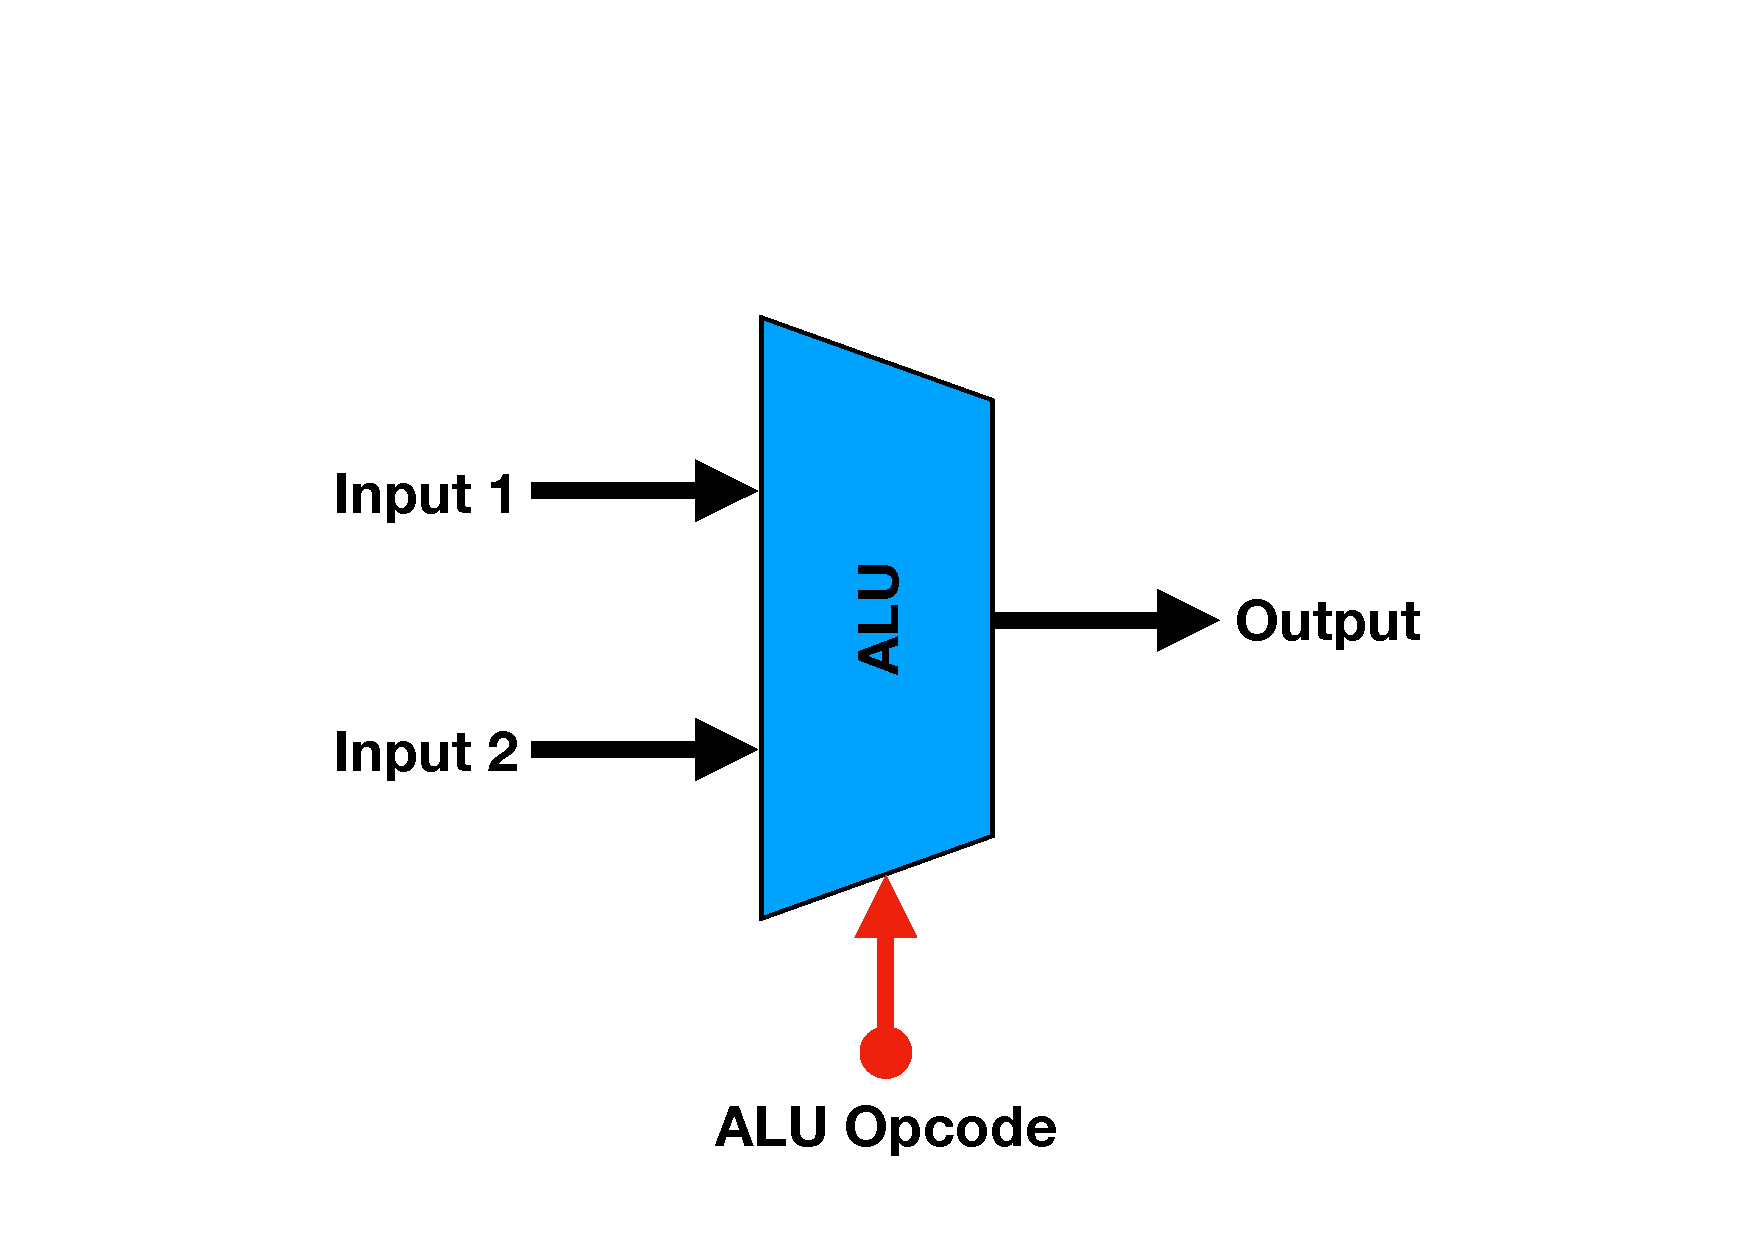
\includegraphics[scale=0.32]{pictures/ALU.pdf}
            \caption{Illustration of the \texttt{ALU} process. The two input contains the operands of the operation to be executed and the output is the result. The ALU opcode (in red) controls which operations the ALU will perform.}
            \label{fig:ALU}
        \end{figure}
    
        \begin{minipage}{\linewidth}
            \begin{lstlisting}[language={[Sharp]C}, caption={A slice of the \texttt{ALU} process SME code. The ALU consists of a large \texttt{switch} statement, with cases for each operation to be performed, which is controlled by the ALU operation code (\texttt{opcode}). },captionpos=b, label = ALU]
...
    protected override void OnTick() {
        switch (m_ALUOP.Value) {
            case 0:
                output.Value = m_ALU_In_1.Data + m_ALU_In_2.Data;   // ADD
                break;
            case 1:
                output.Value = m_ALU_In_1.Data - m_ALU_In_2.Data;   // SUB
                break;
            case 2:
                output.Value = m_ALU_In_1.Data & m_ALU_In_2.Data;   // AND
                break;
            case 3:
                output.Value = m_ALU_In_1.Data | m_ALU_In_2.Data;   // OR
                break;
            case 4:
                ...
        }
    }
            \end{lstlisting}
        \end{minipage}  
        
    
    \subsection{Immediate generator}\label{section:immediategenerator}
        The \texttt{Immediate Generator}, or IMMGEN for short, extracts immediate fields from instructions. This is a pretty large unit since it needs to know where the immediate field is located in every instruction. To make matters worse some immediate fields in the instructions are totally scrambled, so we have to be really careful on how we reconstruct them.
        
        To start we need to be able to identify which type of instruction we are dealing with to know where the immediate field is located. Luckily almost all types of instructions have a unique operation code (for example the I-type has opcode 19), we therefore use a \texttt{switch} statement in the SME code with the opcode in the instruction as a branching condition to identify the instruction type.
        
        Some instructions of same type, only use the lower 6 bits in the immediate field, such as the \texttt{slli} instruction. To accommodate this fact we make use of another \texttt{switch} statement, within the specific case of the first \texttt{switch} statement, that uses the \texttt{funct3} field as branching condition, since this is the unique identifier within the same type of instruction (for example \texttt{opcode} 19, \texttt{funct3} 1 is the \texttt{slli} instruction).
        
        When we know where the immediate field is located it is time to extract it. This is done by shifting the instruction in question to the right, such that the first bit of the immediate field is located at bit index 0 of the 32-bit instruction. Hereafter we do a bitwise AND operation to remove all but the necessary bits (see Section \ref{section:Operators}). It should be noted that in cases, where the immediate field only is 12-bits long we need to perform a shift to the left and then right to retain the sign bit, as 12-bit numbers are not supported by \texttt{C\#} and therefore does not happen automatically, when cast to \texttt{long} type.
        
        If we deal with \texttt{B-} and \texttt{J-type} instructions, we need to be really careful when we reconstruct the immediate field, as the immediate field bits do not lie in a trivial manner. An important thing to note is that in these types of instructions the first bit is not supplied and therefore should not get shifted all the way to the 0'th bit index but should get shifted to the 1'st bit index. This firstly ensures that we only jump by an even number of bytes, as this is where the base index is for the instructions and secondly it effectively doubles the range we can jump instructions.
        
        When the immediate field is constructed it simply gets outputted as a signed 64-bit number. The immediate generator is illustrated in Figure \ref{fig:IMMGEN} and a code segment is shown in Listing \ref{IMMGEN}.
        
        
        \begin{figure}[h!]
            \centering
            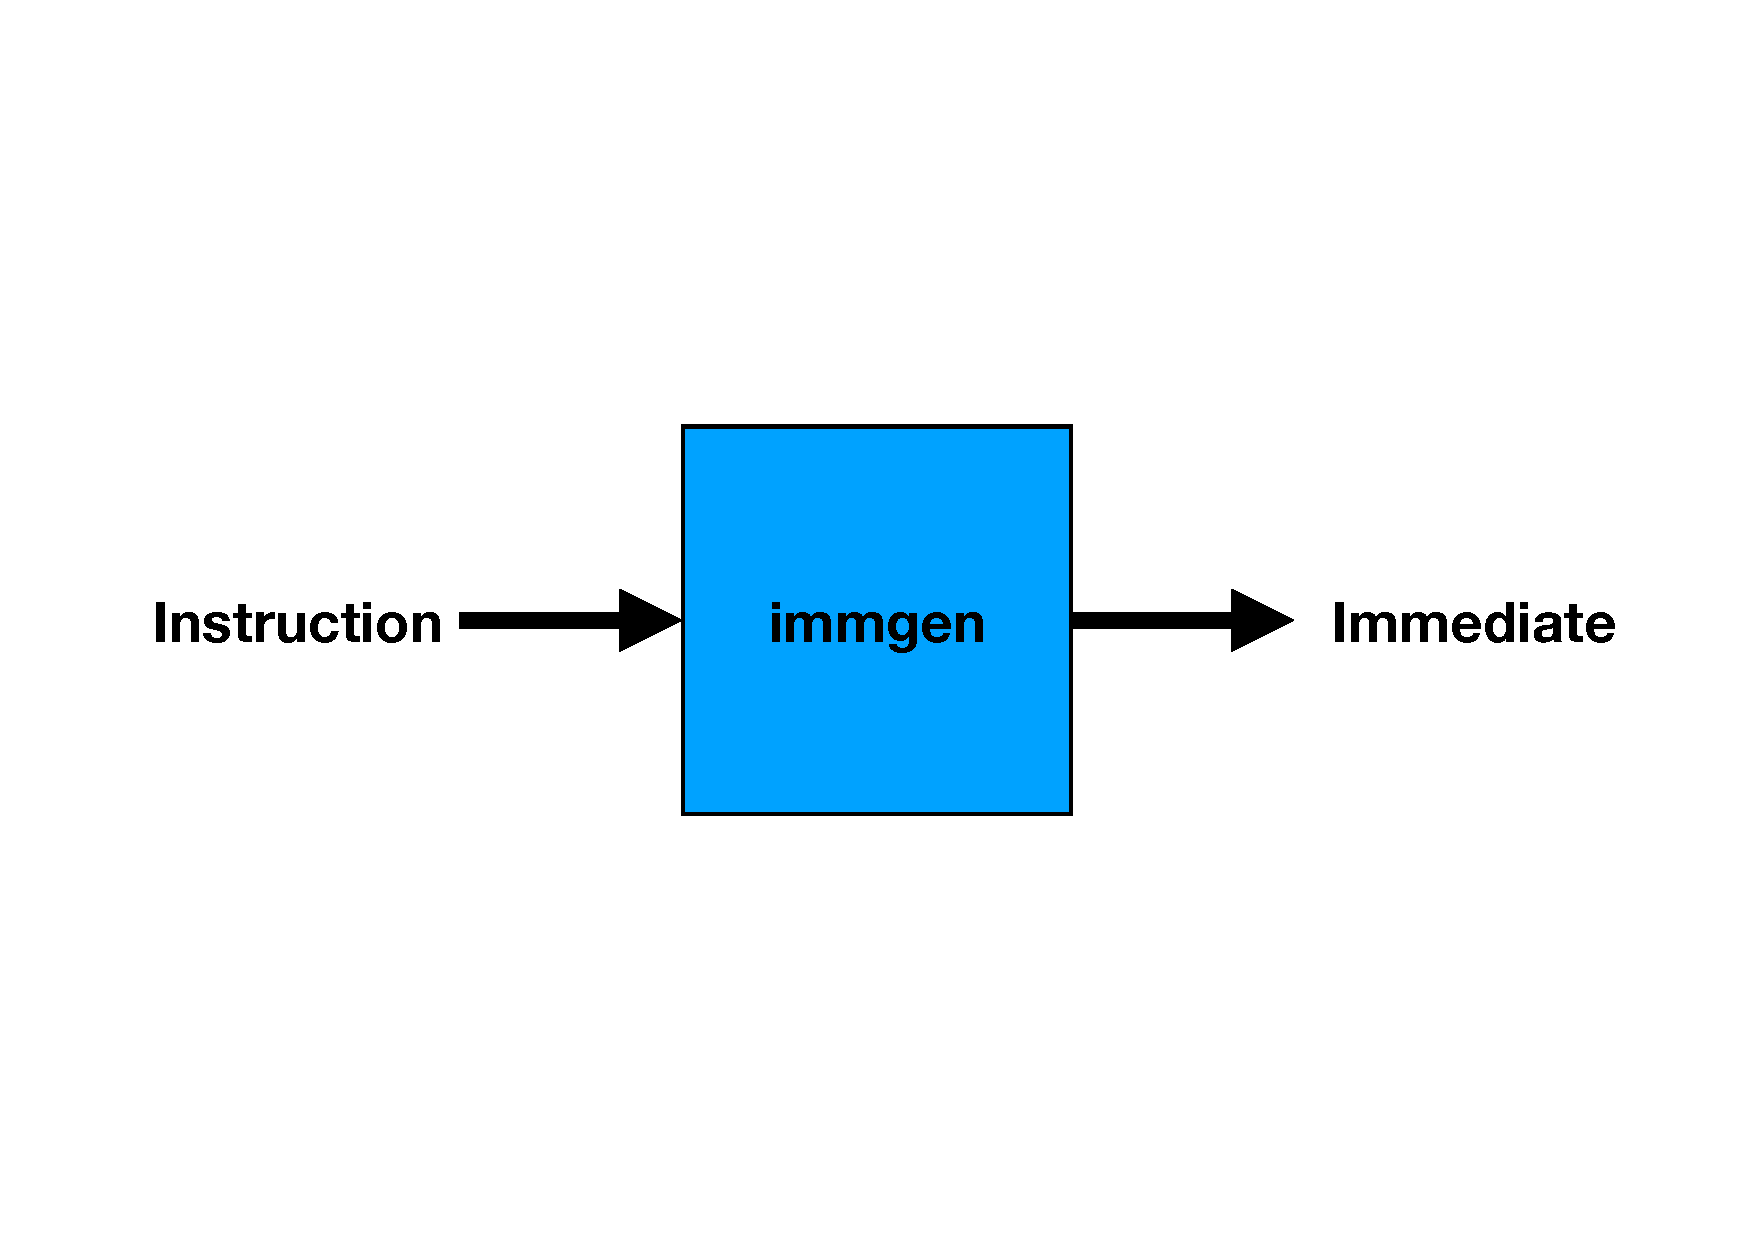
\includegraphics[scale=0.35]{pictures/IMMGEN.pdf}
            \caption{Illustration of the \texttt{immediate generation} process, taking an instruction as input. It then extracts the immediate field, which it outputs. }
            \label{fig:IMMGEN}
        \end{figure}
    
        \begin{minipage}{\linewidth}
            \begin{lstlisting}[language={[Sharp]C}, caption={A slice of the \texttt{IMMGEN} process SME code. We first extract the opcode and funct3 fields from the instruction and put them in a variable. We then use a \texttt{switch} statement and the opcode to determine what type of instruction we are dealing with. Since some instructions of same type like \texttt{slli} only use the lower 6 bits in the immediate field (shamt field), we need another switch statement to tell these apart using the funct3 field. Lastly we construct the immediate and output it . Note that in line 18 we make use of a little hack to retain the sign bit of a 12 bit number since it is not supported in \texttt{C\#}},captionpos=b, label = IMMGEN]
...
    protected override void OnTick() {
        uint Opcode = m_instruction.Current & (uint)0x7F;
        uint funct3 = m_instruction.Current >> 12 & (uint)0x7;
            
        switch(Opcode) {
            ...
            case 19:                                        // I-format
                switch (funct3) {
                    ...
                    case 5:
                        temp1 = m_instruction.Current >> 20 & (uint)0x3F;
                        temp0 = (long)temp1;
                        output.Immediate = temp0;
                        break;
                    default:
                        temp1 = m_instruction.Current >> 20 & (uint)0xFFF;
                        short temp5 = (short)((short)(temp1 << 4) >> 4);
                        temp0 = (long)temp5;
                        output.Immediate = temp0;
                        break;
                }
            break;
            case 27:                                        // I-format Word
                ....
        }
    }
            \end{lstlisting}
        \end{minipage} 
\newpage
    \subsection{Data Memory}
        The \texttt{Data Memory}, or DM for short, is the main data storage unit of the CPU, as it can contain much more data than the register. The data memory is very similar to the instruction memory, as it is also little-endian addressed and is constructed from a byte array. The processor can either read or write from the data memory unit once per clock cycle.
        
        Because of this fact the data memory needs control signals, which manages read and write access. To support data of varying size an additional control signal has been added to distinguish between double word, word, short and byte access. Since unsigned versions of the \texttt{load} instructions also needs to be supported, this functionality is added to the size control signal.
        
        As the data memory communicates with the register, which is big-endian addressed and every element is 64-bit a translation needs to happen between these formats.
        
        In SME a process is created that contains a byte array. To support 64-bit numbers the array has to be larger than 8 bytes if a single number has to be stored. Otherwise the sizing is irrelevant if made big enough and is divisible by eight. In this implementation the array is 2000 bytes long.
        
        To distinguish between the read and write states an \texttt{if/else} statement is used. For the branching condition, two control signals are used to determine whether a read or write should be performed. When reading or writing the size of the data needs to be known, such that a correct translation between big- and little-endian formats can take place. To this end a \texttt{switch} statement is used, with cases for each data size scenario. Furthermore cases for handling unsigned reads has been added.
        
        The read and write address gets calculated by the ALU and the data is supplied by the second register output line. If the read control is enabled the data memory will output the specified data. The data memory is illustrated in Figure \ref{fig:DM} and a code segment is shown in Listing \ref{DM}.
        
        \begin{figure}[h!]
            \centering
            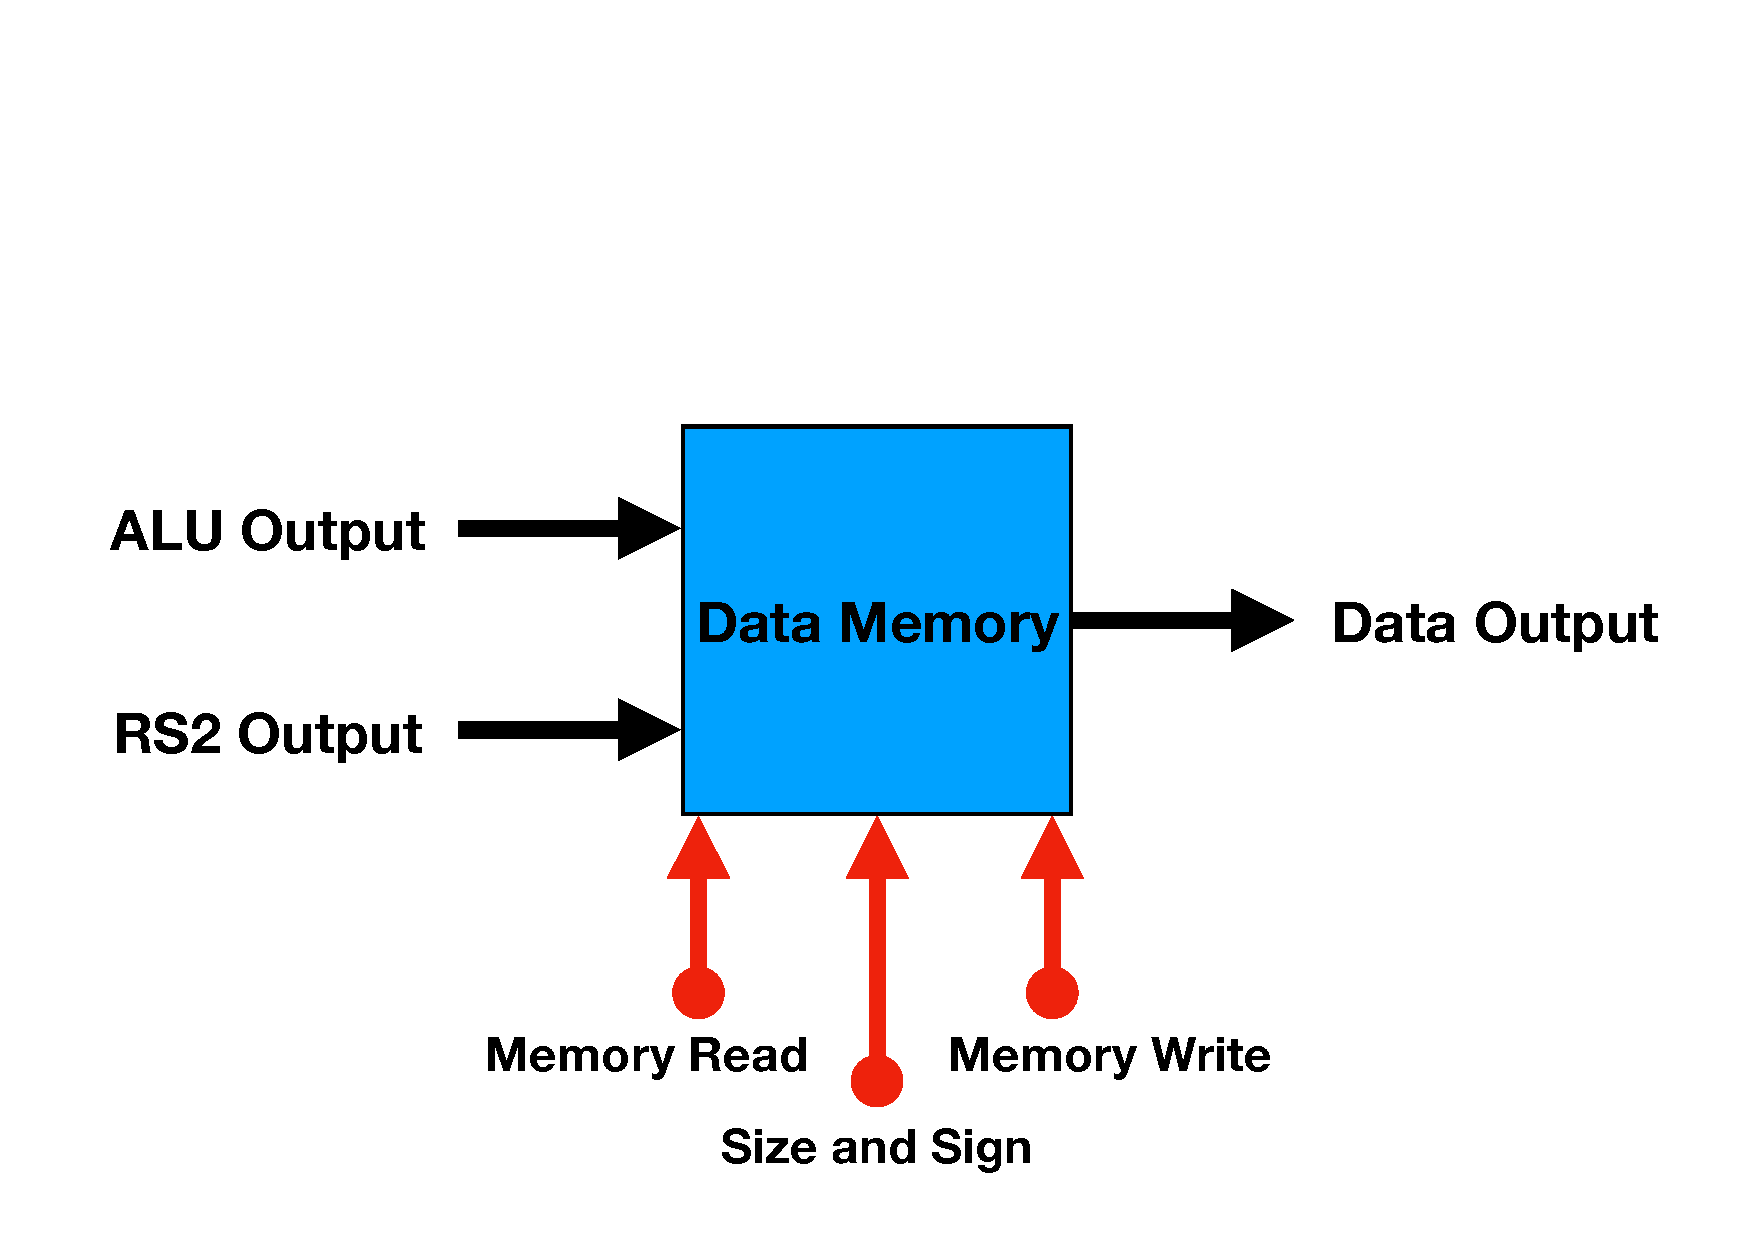
\includegraphics[scale=0.29]{pictures/DM.pdf}
            \caption{Illustration of the \texttt{Data Memory} process. The target address is calculated in the ALU and data to be written outputted from register 2, which the unit takes as input. Controls signals are marked in red and consists of \texttt{Memory Read}, \texttt{Memory Write} and \texttt{Size and Sign}. It then outputs the read data or 0 if both \texttt{Memory Read} and \texttt{Memory Write} are deasserted.}
            \label{fig:DM}
        \end{figure}
    
        \begin{minipage}{\linewidth}
            \begin{lstlisting}[language={[Sharp]C}, caption={A slice of the \texttt{Data Memory} process SME code. Similar to the instruction memory, the data memory consists of a byte array, which we made 2000 elements long in this case. As there can only be read or written to the data memory once per clock cycle, we simply construct an \texttt{if/else} statement, which uses control signals to determine the procedure to be done. Both the read and write procedures needs to know the size and sign of the data to be loaded or written. Therefore a \texttt{switch} statement has been added to both outcomes, which uses \texttt{SizeAndSign} control signal to choose between the cases. When reading the data from memory we need to remember that it is little-endian addressed  so before we output the value the bits need to be shuffled around in the correct order, so the correct value is added to the register, as that is big-endian. When writing the data the opposite need to happen, so a big-endian value need to be converted to a little-endian one. If both read and write control signals are deasserted I choose to output 0.},captionpos=b, label = DM]
...
    byte[] Data_Memory = new byte[2000];
            
    protected override void OnTick() {
        if (m_MemRead.Enable) {
            ...
            switch (m_SizeAndSign.Value) {
                ...
                case 1: // load word
                    temp0 =
                    Data_Memory[m_Address.Value] | Data_Memory[m_Address.Value + 1] << 8
                                                 | Data_Memory[m_Address.Value + 2] << 16
                                          | (sbyte)Data_Memory[m_Address.Value + 3] << 24;
                    break;
                case 2: // load short
                    ...
            }
            output.Data = temp0;
        }
        else if (m_MemWrite.Enable) {
            switch (m_SizeAndSign.Value) {
                ...
                case 2:
                    Data_Memory[m_Address.Value]     = (byte)(m_Data_input.Data      & 0xFF);
                    Data_Memory[m_Address.Value + 1] = (byte)(m_Data_input.Data >> 8 & 0xFF);
                    break;
                case 3:
                    Data_Memory[m_Address.Value] = (byte)(m_Data_input.Data & 0xFF); 
                    break;
            }
        }
        else {
            output.Data = 0;
        }
    }
            \end{lstlisting}
        \end{minipage} 
    
    \subsection{Go to Unit}
        To support the RISC-V branching and jump instructions a special unit called \texttt{Go To} was created. The purpose of this unit is to do the logical comparison between the specified registers. For example if the \texttt{branch if equal} (\texttt{BEQ}) instruction is given, the unit will check if the values in the specified registers are equal and outputs logical \texttt{true} or \texttt{false} depending on the result.
        
        In the SME implementation a simple \texttt{switch} statement is used. Each case represent the comparison to be done by a given instruction, where the case branching is controlled by a control line. The result is then outputted. The Go To unit is illustrated in Figure \ref{fig:GOTO} and a code segment is shown in Listing \ref{GOTO}.
        
        
        \begin{figure}[h!]
            \centering
            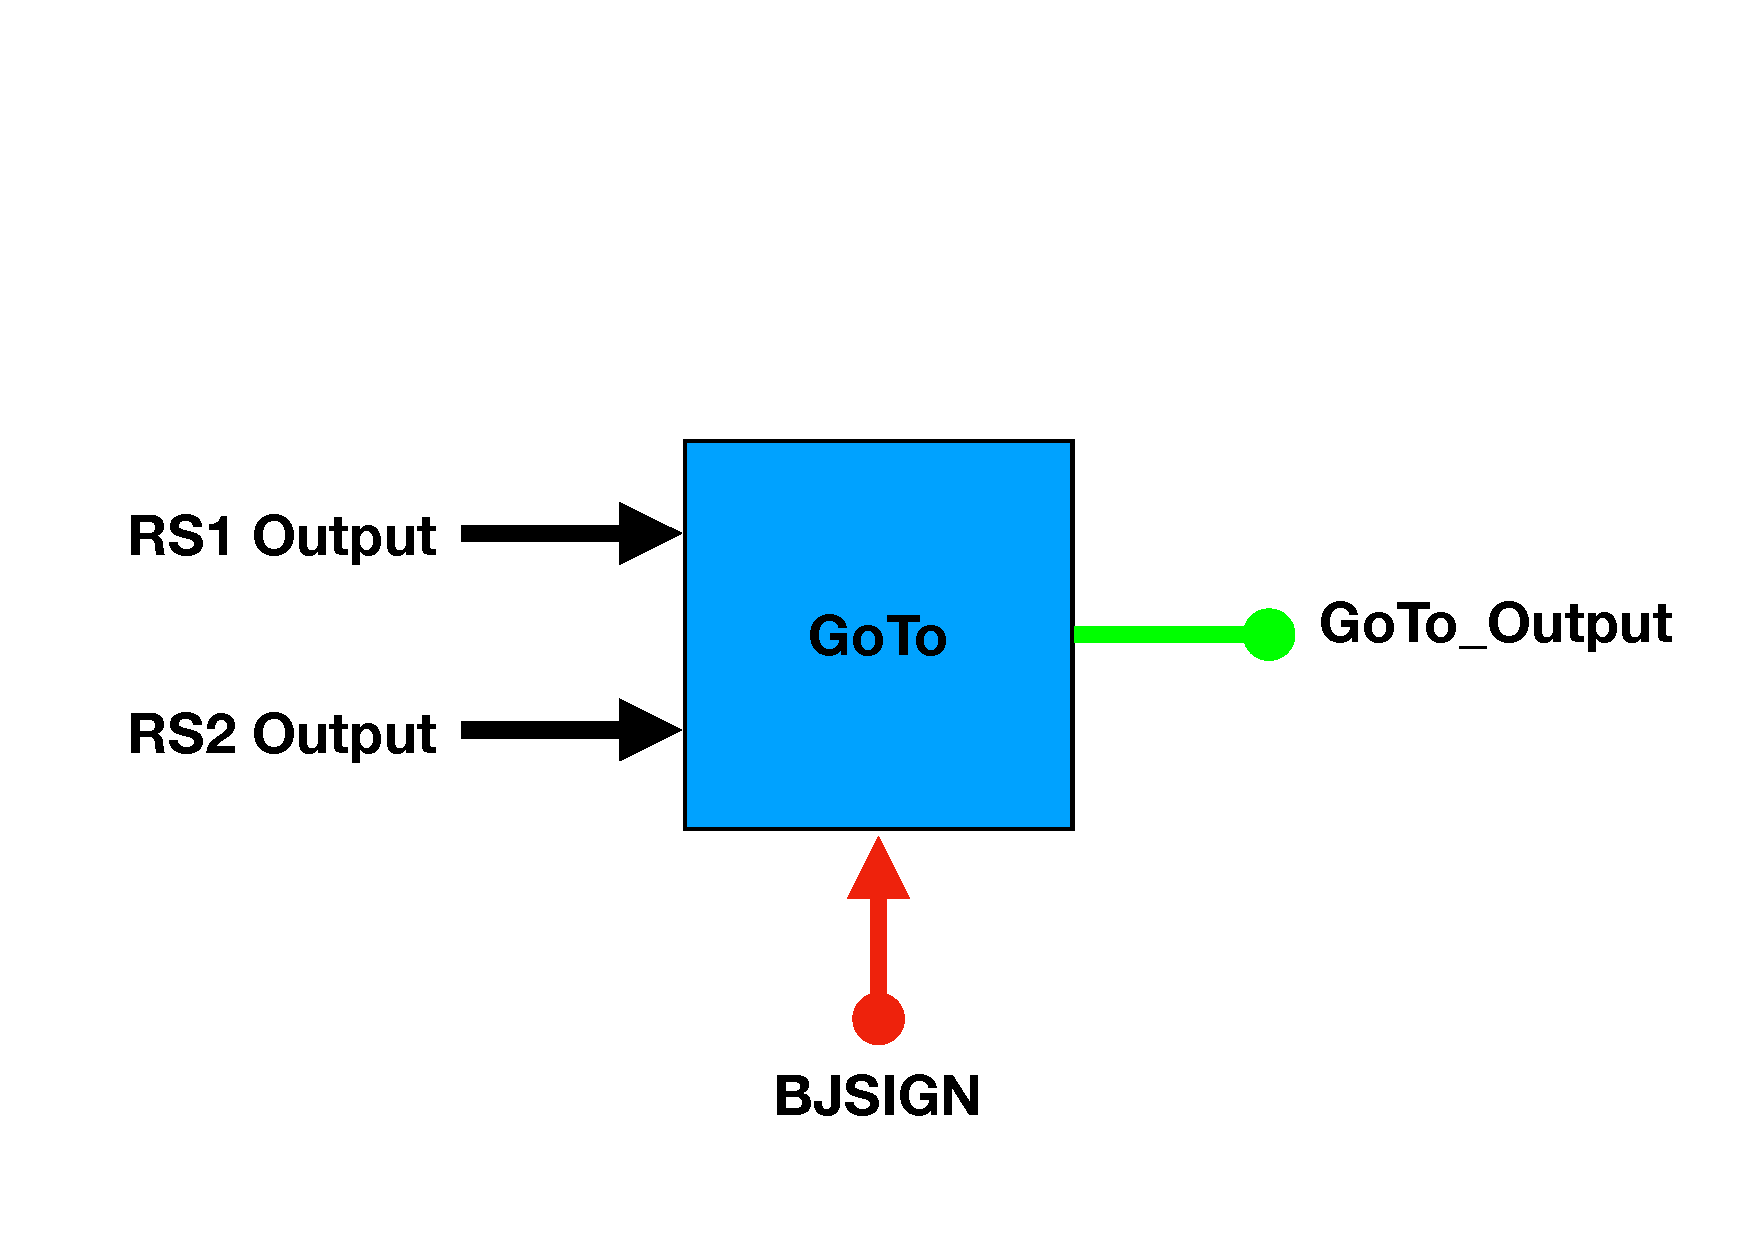
\includegraphics[scale=0.35]{pictures/GOTO.pdf}
            \caption{Illustration of the \texttt{Go To} process. As input it uses the two output lines from the register. It has one control line in red and one output line in green.}
            \label{fig:GOTO}
        \end{figure}
    
        \begin{minipage}{\linewidth}
            \begin{lstlisting}[language={[Sharp]C}, caption={A slice of the \texttt{Go To} process SME code. The unit consists of a \texttt{switch} statement, where each case does the comparison relevandt to the branching instruction. The conditional operator \texttt{?} is used for the comparison (the syntax goes as follows \texttt{condition ? If true return this : If false return this}).},captionpos=b, label = GOTO]
...
    protected override void OnTick() {
        switch (m_BJSIGN.Value) {
            case 0:
                output.Value = (m_RS1.Data == m_RS2.Data) ? true:false; // BEQ
                break;
            case 1:
                output.Value = (m_RS1.Data != m_RS2.Data) ? true:false; // BNE
                break;
            case 2:
                ...
        }
    }
            \end{lstlisting}
        \end{minipage}
    
    \subsection{Multiplexer}
        To select between multiple lines we make use of a \texttt{multiplexer}, or mux. It is a fairly simple process that only consists of a \texttt{switch} statement, where each case corresponds to an input to output. The cases then gets selected depending on the control line. The multiplexer is illustrated in Figure \ref{fig:MUX} and a code segment is shown in Listing \ref{MUX}.
        
        \begin{figure}[h!]
            \centering
            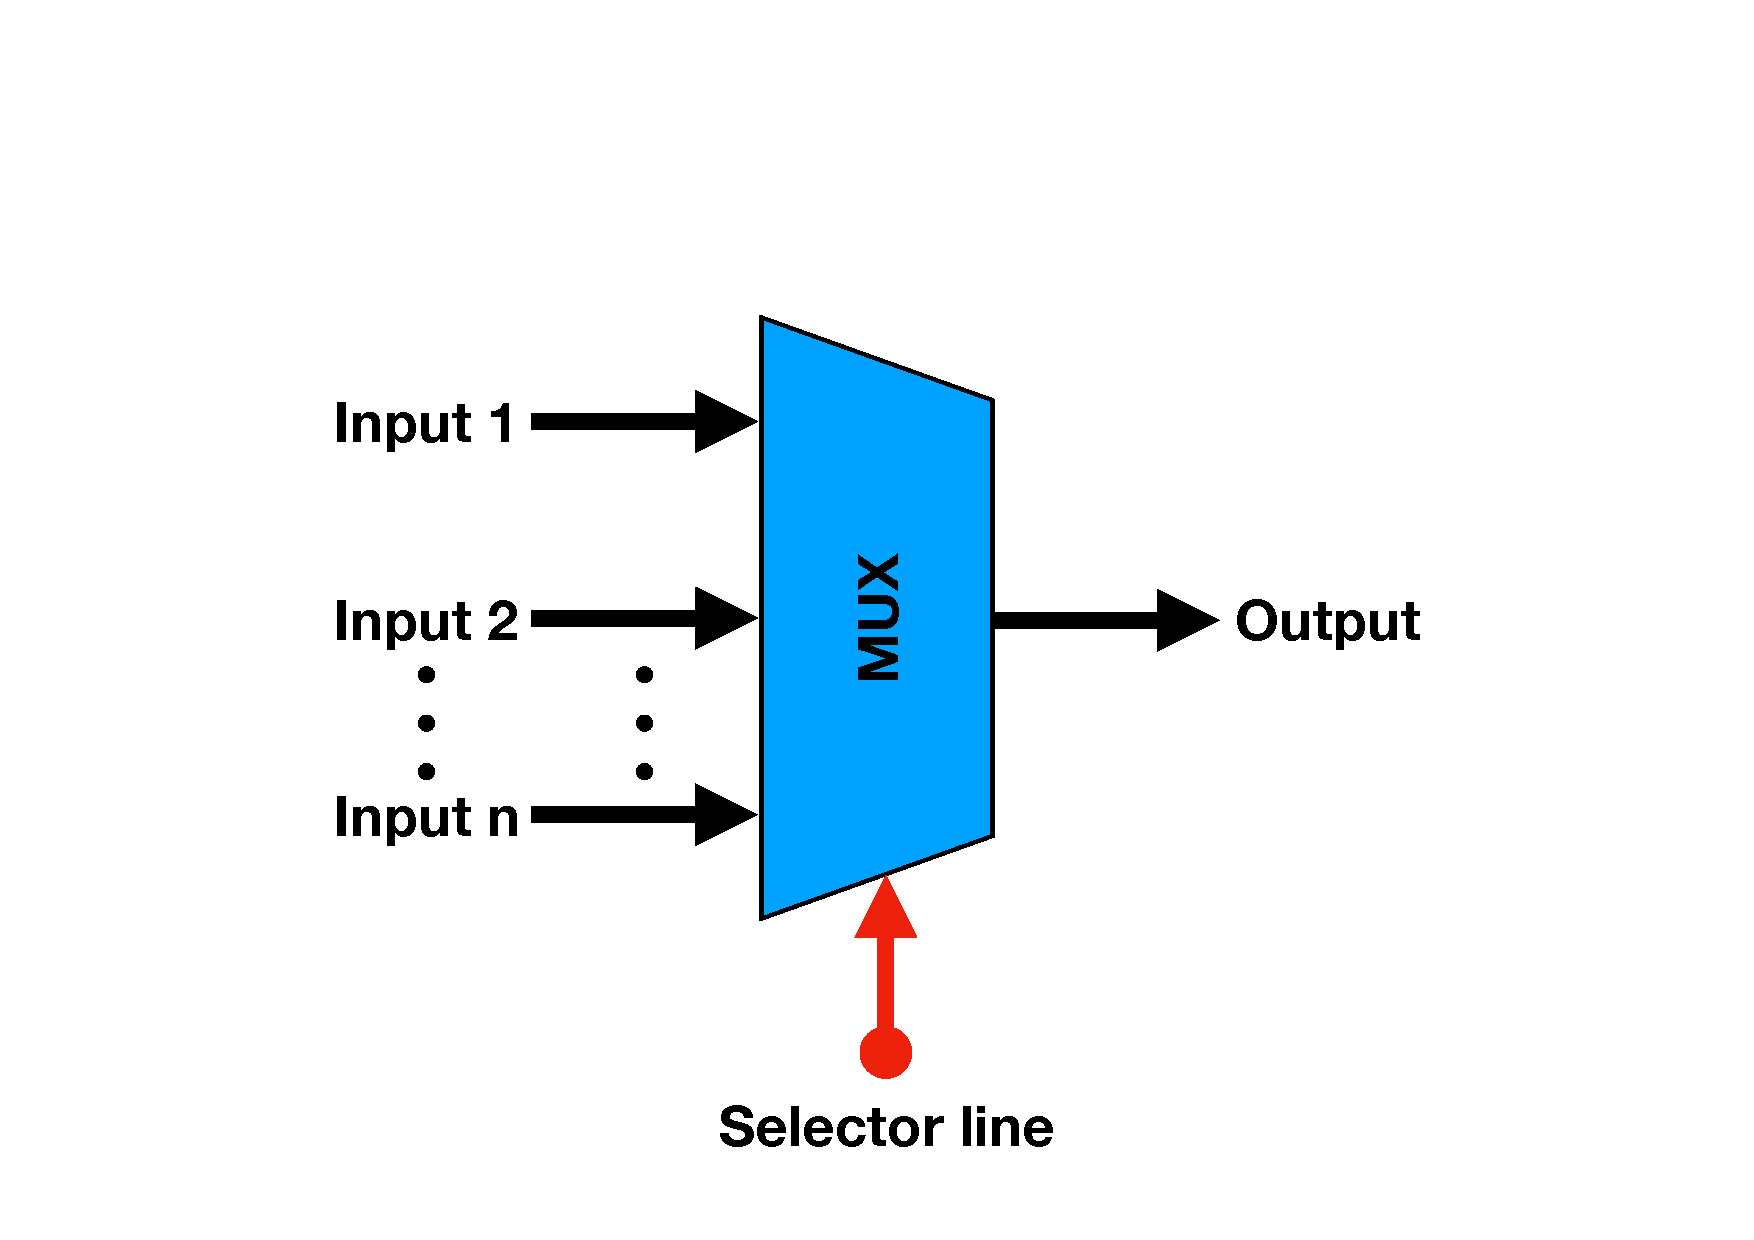
\includegraphics[scale=0.35]{pictures/MUX.pdf}
            \caption{Illustration of the \texttt{Multiplexer} process. An arbitrary amount of input can be given, where the output i selected by the red control line. }
            \label{fig:MUX}
        \end{figure}
    
        \begin{minipage}{\linewidth}
            \begin{lstlisting}[language={[Sharp]C}, caption={An example of a \texttt{Multiplexer} process SME code. The whole multiplexer simply consists of a \texttt{switch} statement that selects an input to output dependent on \texttt{SelectBus}.},captionpos=b, label = MUX]
...
    protected override void OnTick() {
        switch (SelectBus) {
            case 0:
                Mux_output = input1;
                break;
            case 1:
                Mux_output = input2; 
                break;
            case 2:
                Mux_output = input3; 
                break;
        }
    }
            \end{lstlisting}
        \end{minipage}
\newpage
    \subsection{Write Back Unit}
        When wire-ring the processor there is going to form a second closed loop between the register and data memory. As with the closed loop between the program counter and Next unit, there has to be a clocked process somewhere in the loop. For this reason a clocked write back process is introduced. It works exactly the same as the program counter, which read the contents of a bus that contained data from the previous clock cycle and got outputted unchanged. 
        
        It may seem that this could cause problems, but as the data output from this unit gets written to the register as the first thing, instructions will never access old data.  The \texttt{Write Back} unit is illustrated in Figure \ref{fig:WB} and a code segment is shown in Listing \ref{WB}.
        \begin{figure}[h!]
            \centering
            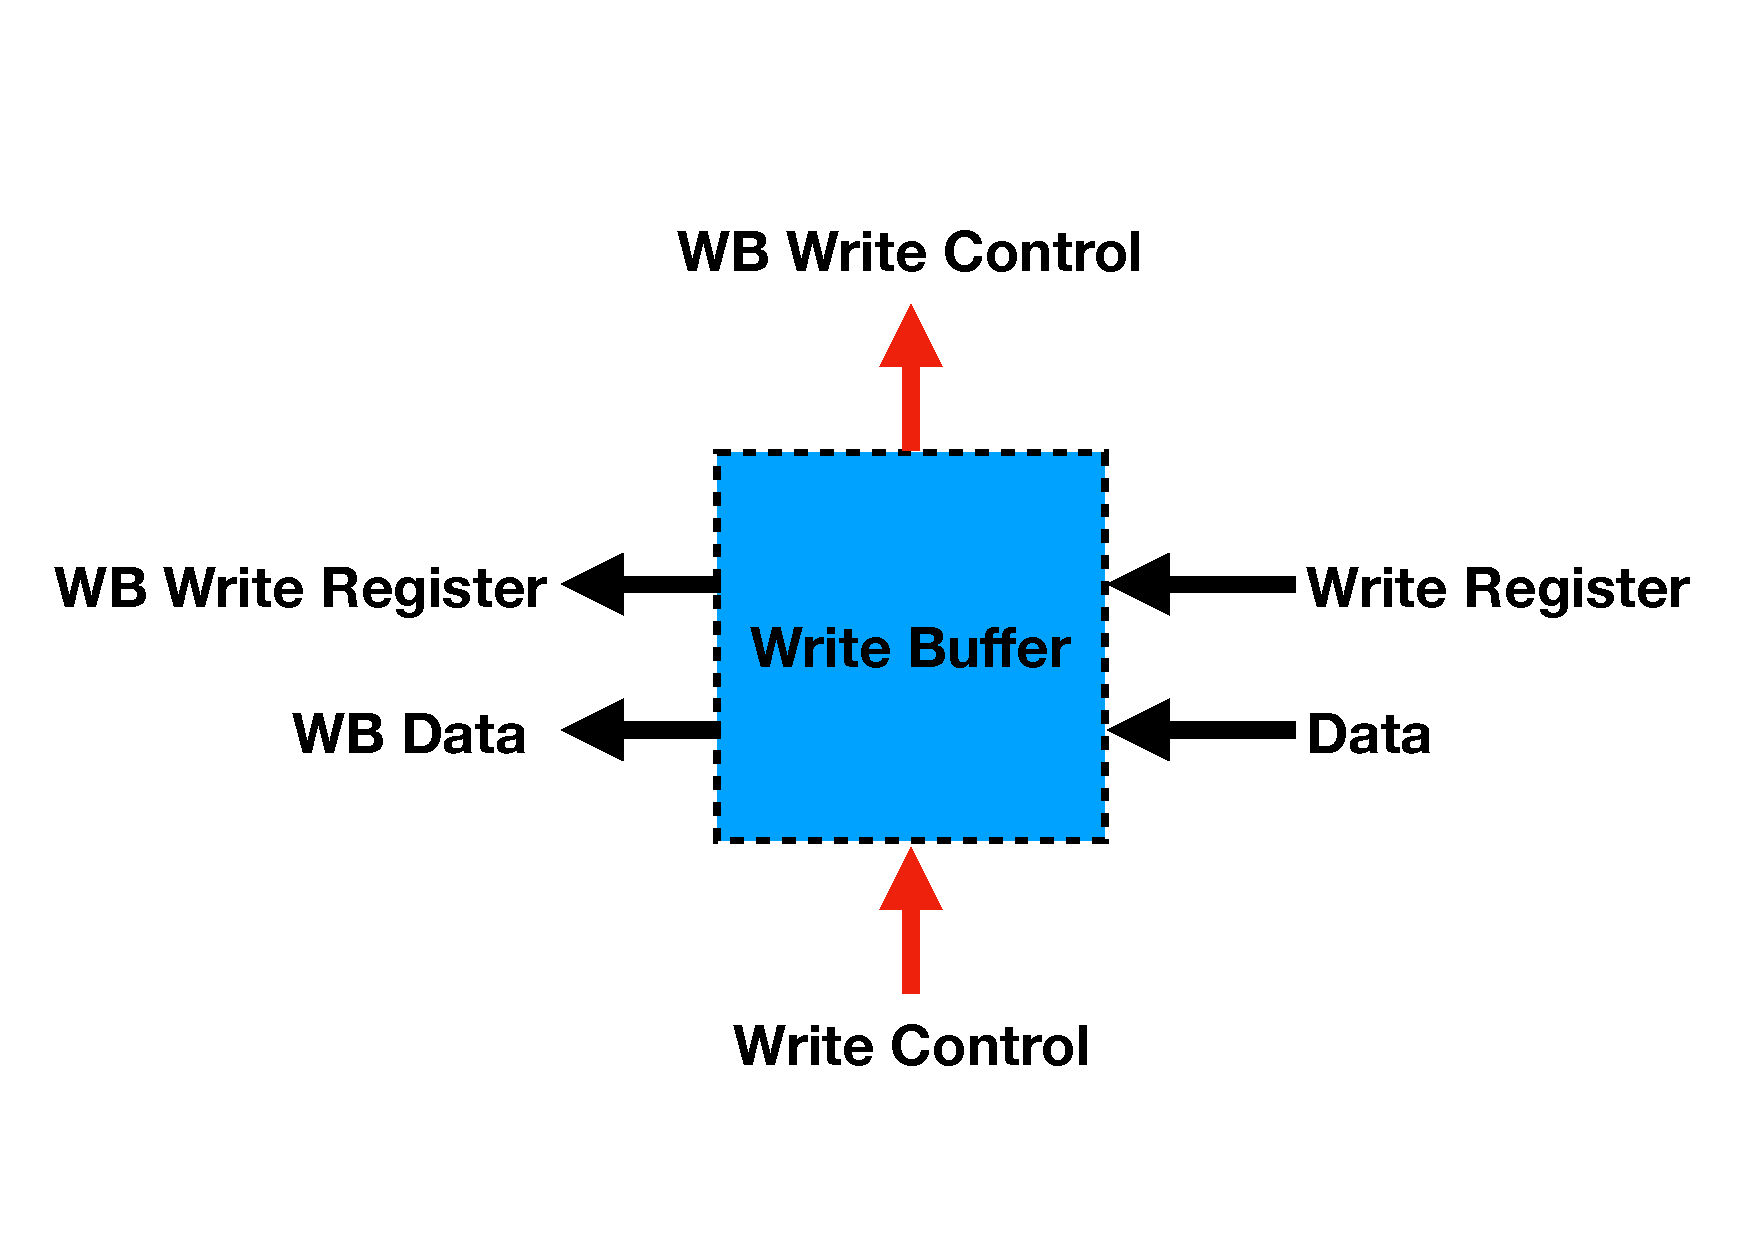
\includegraphics[scale=0.35]{pictures/WB.pdf}
            \caption{Illustration of the \texttt{Write Back} process. It has 3 input \texttt{Data}, \texttt{Write Register} and \texttt{Write control}. These input gets outputted unchanged to their respective output buses. The dashed square indicates a clocked process.}
            \label{fig:WB}
        \end{figure}
    
        \begin{minipage}{\linewidth}
            \begin{lstlisting}[language={[Sharp]C}, caption={A slice of the \texttt{Write Back} process SME code. It contains 3 variables, which will hold the incomming values, which gets outputted unchanged in the same clock cycle.},captionpos=b, label = WB]
...
    long WB_Data_Hold;
    uint WB_RegisterWrite_Hold;
    bool WB_WriteControl_Hold;
    
    protected override void OnTick() {
        WB_Data_Hold = m_write_data.Data;
        WB_RegisterWrite_Hold = m_write_register.Address;
        WB_WriteControl_Hold = m_write_control.Enable;
    
        m_WB_Data.Data = WB_Data_Hold;
        m_WB_WriteRegister.Address = WB_RegisterWrite_Hold;
        m_WB_WriteControl.Enable = WB_WriteControl_Hold;
    }
            \end{lstlisting}
        \end{minipage} 
    
    \subsection{AND gate unit}
        To make use of a trick inspired from the RISC-V implementation in chapter 4 of \cite{riscVbook} an AND gate unit has been implemented. The purpose of this unit is to check whether branching or jumping instructions are given. If such instructions are taking place a control signal is asserted. The AND gate only returns true if the branching condition from the \texttt{Go To} gate returns true. This result can now be feed to a multiplexer which chooses whether to run next instruction or jump in the instruction memory. The \texttt{AND} unit is illustrated in Figure \ref{fig:AND} and a code segment is shown in Listing \ref{AND}.
        
        \begin{figure}[h!]
            \centering
            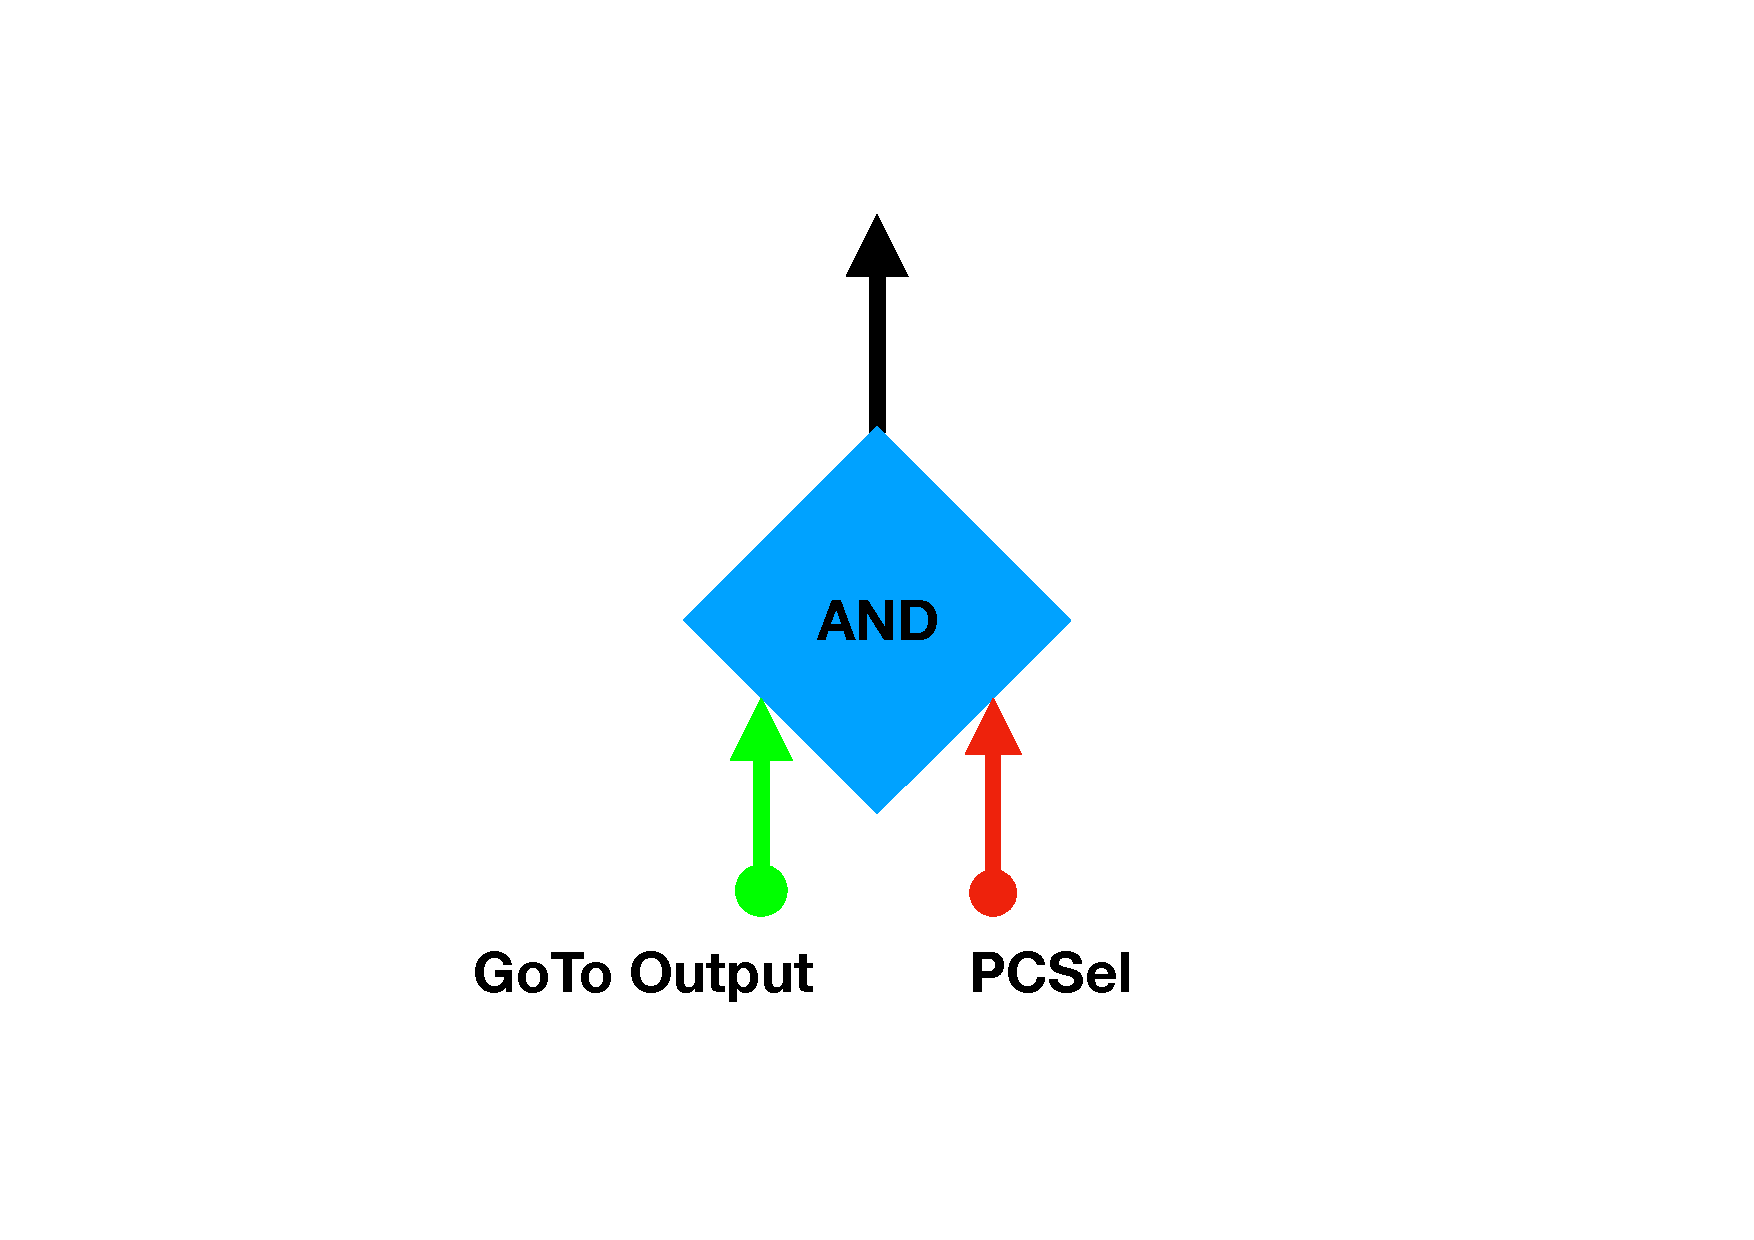
\includegraphics[scale=0.35]{pictures/AND.pdf}
            \caption{Illustration of the \texttt{AND gate} process. It has two input one from the \texttt{Go To} unit and one from the \texttt{control unit} named \texttt{PCSel}. The output is then the result of the logical AND operation between the two input.}
            \label{fig:AND}
        \end{figure}
    
        \begin{minipage}{\linewidth}
            \begin{lstlisting}[language={[Sharp]C}, caption={A slice of the \texttt{AND gate} process SME code. It simply calculates the logical AND of two input and outputs the result.},captionpos=b, label = AND]
...
    protected override void OnTick() {
        Output.Value = m_Input_1.Value && m_Input_2.Value;
    }
            \end{lstlisting}
        \end{minipage} 
        
    \subsection{Control}
        The final unit that is to be shown is the \texttt{Control} unit. This is quite a substantial unit, as its function is to correctly set the values for the control lines for all 49 instructions. What the values look like will be discussed in Section \ref{section:Datapaths}. For now the SME implementation will be covered.
        
        This unit uses a similar solution for instruction detection, as the \texttt{Immediate Generator} (see Section \ref{section:immediategenerator}). To identify the current instruction the \texttt{opcode}, \texttt{funct3} and \texttt{funct7} fields are extracted from the 32-bit instruction input and put in their respective variables. All 3 fields are used this time, as every instruction needs to be identified to correctly set the control lines.
        
        Multiple \texttt{switch} statements are layered for instruction detection. The first \texttt{switch} uses the \texttt{opcode} to determine the type of instruction that is currently running. Say a R-type instruction has been identified. Most control lines can be set here, as only the control line for the ALU is different between the R-type instructions. To set the last control line a second \texttt{switch} statement is used with the \texttt{funct3} field as branching condition to identify which R-type instruction is given. Since some R-type instructions has the same \texttt{funct3} code, a third \texttt{switch} statement is required to differentiate these.
        
        When an instruction as been identified the control lines are set to the correct values and outputted. The \texttt{Control} unit is illustrated in Figure \ref{fig:CONTROL} and a code segment is shown in Listing \ref{CONTROL}.
        
        
        \begin{figure}[h!]
            \centering
            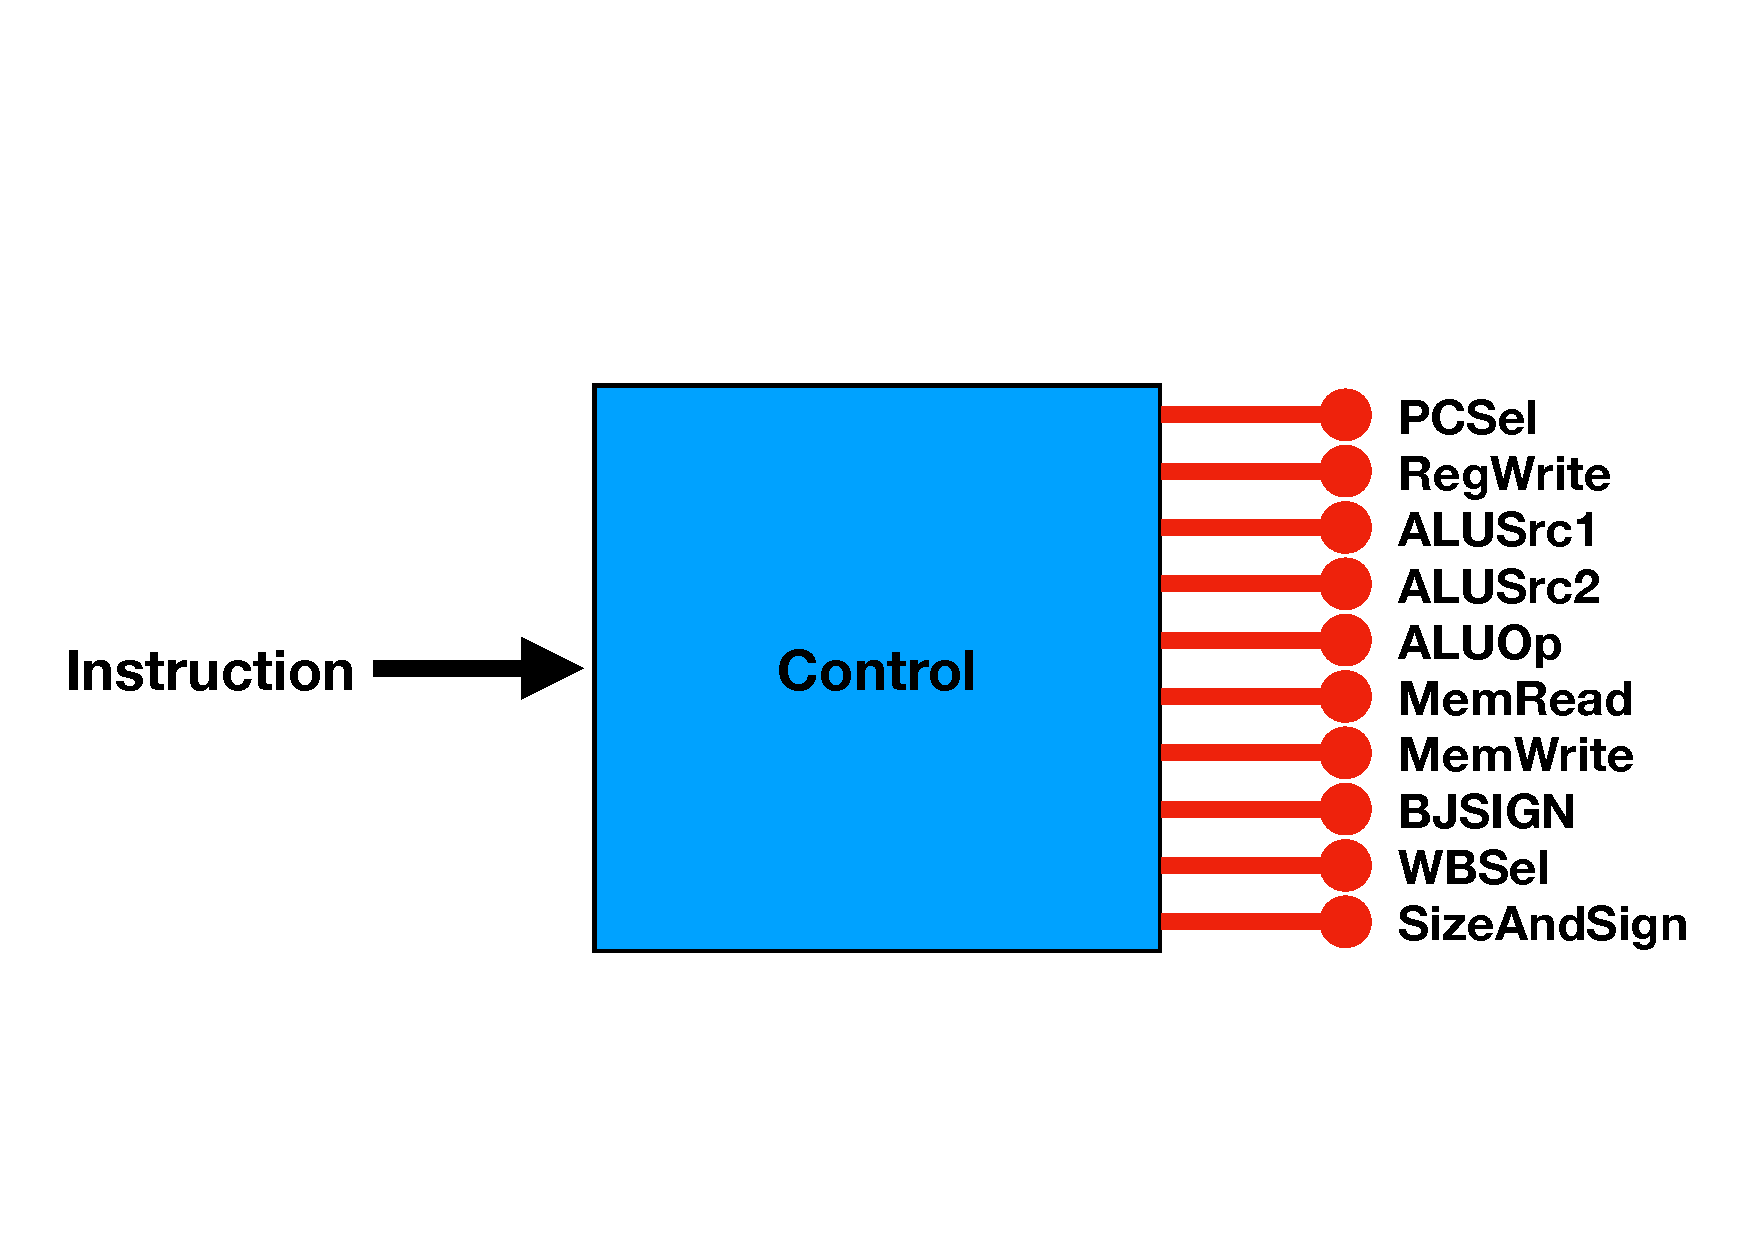
\includegraphics[scale=0.35]{pictures/CONTROL.pdf}
            \caption{Illustration of the \texttt{Control} process. It takes a 32-bit instruction as input and sets the control lines for the respective instruction.}
            \label{fig:CONTROL}
        \end{figure}
    
        \begin{minipage}{\linewidth}
            \begin{lstlisting}[language={[Sharp]C}, caption={A slice of the \texttt{Control} process SME code. First 3 varibles are declared for the extracted \texttt{opcode}, \texttt{funct3} and \texttt{func7} fields. They are then used in the following \texttt{switch} statements to correctly identify the given instruction. Finally the control lines are set with the values for the respective instruction.},captionpos=b, label = CONTROL]
...
    protected override void OnTick() {
        uint Opcode = m_instruction.Current       & (uint)0x7F;  
        uint funct3 = m_instruction.Current >> 12 & (uint)0x7;  
        uint funct7 = m_instruction.Current >> 25 & (uint)0x7F;
        switch (Opcode) {
            ...
            case 51:                            // R-format
                PCSel.Value = false;
                RegWrite.Enable = true;
                ALUSrc1.Enable = false;
                ALUSrc2.Enable = false;
                BJSIGN.Value = 0;
                SizeAndSign.Value = 0;
                MemWrite.Enable = false;
                MemRead.Enable = false;
                WBSel.Value = 0;
                
                switch (funct3) {
                    case 5:
                        switch (funct7) {
                            case 0:                         // ADD
                            ALUOP.Value = 0;
                            break;
                        case 32:                        // Subtract
                            ALUOP.Value = 1;
                            break;
                        }
                        break;
                    ...
            ...
        }
    }
            \end{lstlisting}
        \end{minipage} 
\newpage
\section{Single Cycle RISC-V datapaths}\label{section:Datapaths}
    In Section \ref{section:riscunits} all necessary units for the RISC-V implementation were covered. The final step is to connect all units and define the instruction datapaths. The datapath is defined as the path an instruction takes through the RISC-V implementation. The full implementation is illustrated in Figure \ref{fig:RISCV}. 
    
    The unit that determines what path an instruction takes is the control unit. By modifying the values in the control signals, the path an instruction takes can be manipulated. Since the different types of instructions need to follow a very specific path, we need to design the control unit such that the correct paths gets taken.
    
    \begin{figure}[h!]
        \hspace*{-3.8cm}
        \centering
        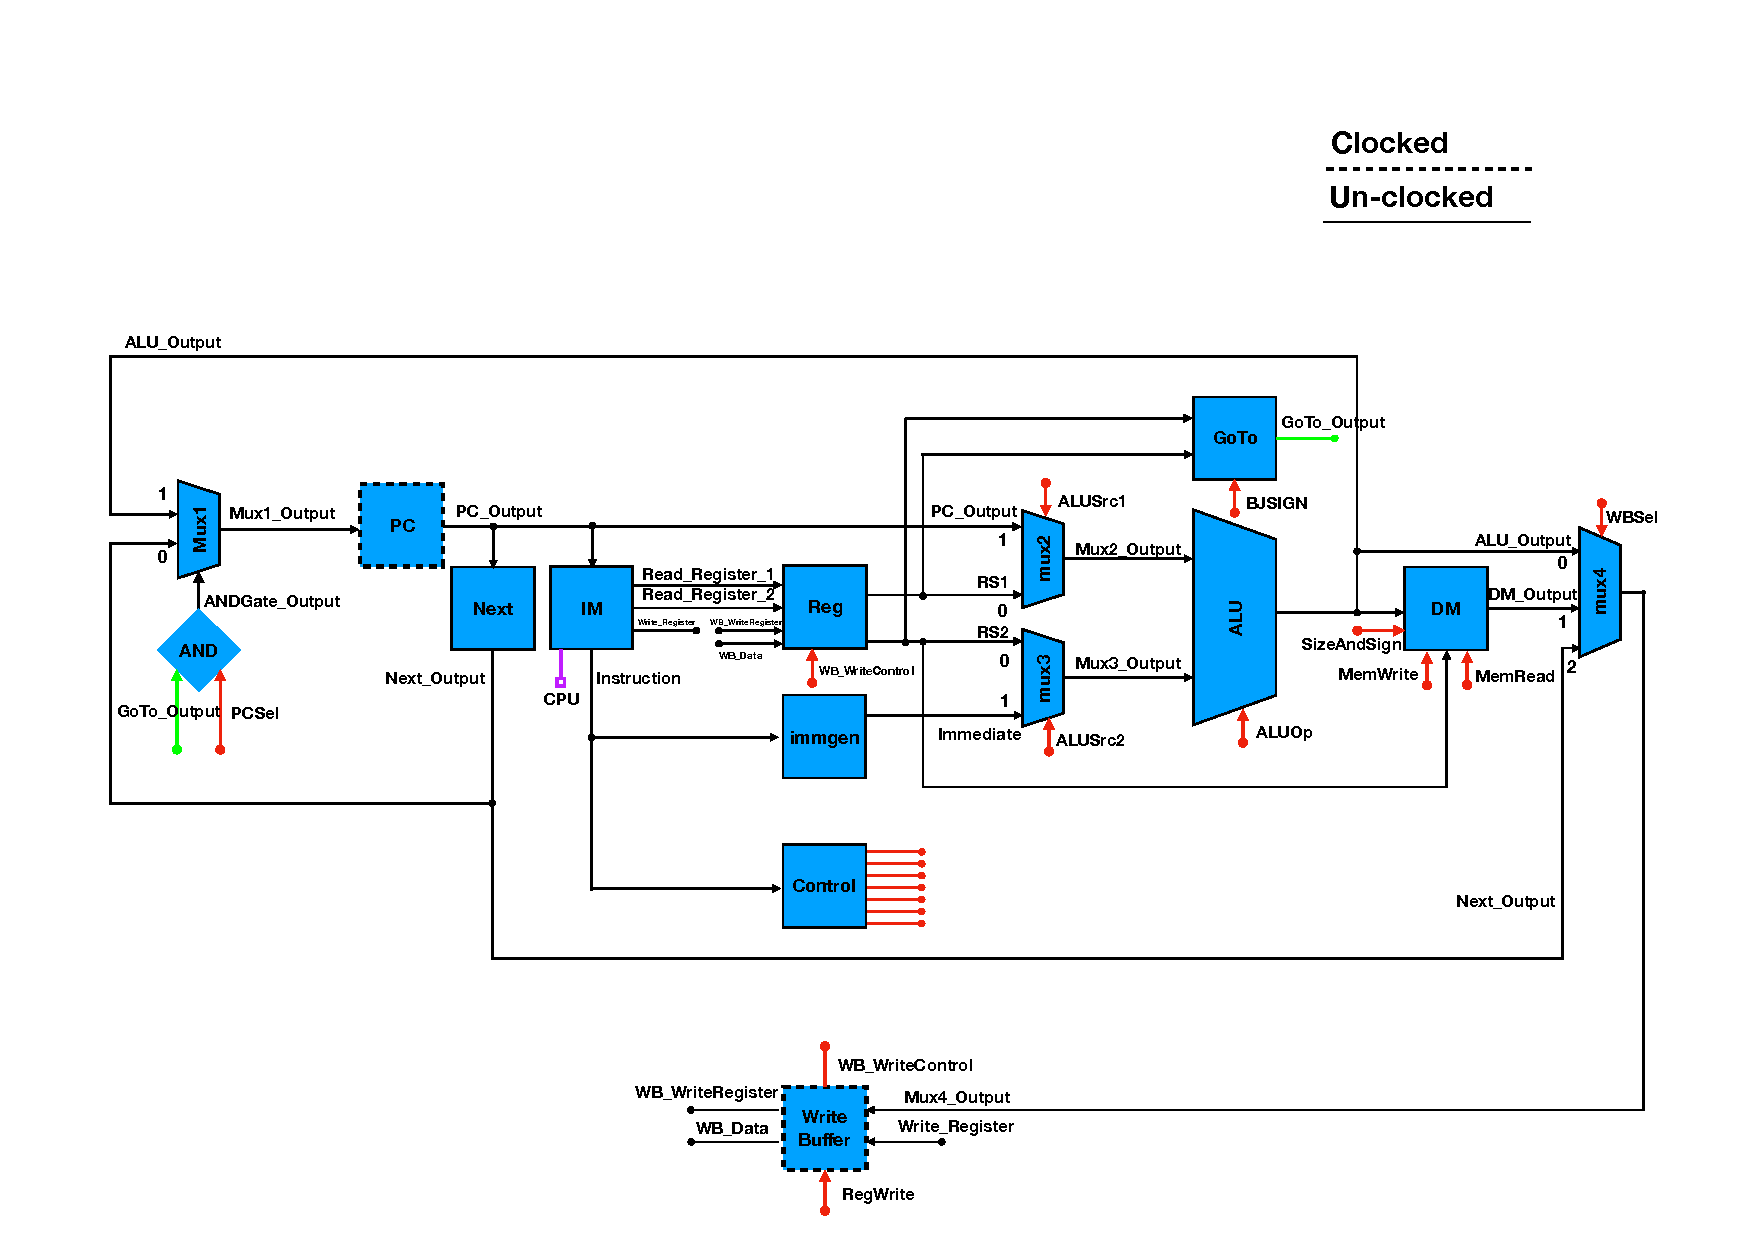
\includegraphics[scale=0.8]{pictures/RISCV.pdf}
        \caption{}
        \label{fig:RISCV}
    \end{figure} 

    \subsection{Supporting R-Format instructions}\label{section:Rformat}
        All R-format instructions perform some arithmetic or logical operation on 2 operands in the register and saves the result back into some specified register. For that to take place two registers has to be read and sent to the \texttt{ALU} where the operation takes place. Therefore the control signals controlling \texttt{mux2} and \texttt{mux3} needs to be deasserted, such that they output the values read in the two registers. 
        
        The control signal that controls the \texttt{ALU} is then set to the operation to be performed by the R-type instruction. The write back to the register is then determined by \texttt{mux4}. Since the result of the \texttt{ALU} is to be written back into some specified register, input 0 of \texttt{mux4} is selected and the write control line of the register is asserted.
        
        Finally the \texttt{PCSel} line is deasserted such that address of the next instruction is inputted to the program counter, since R-format instructions do not perform any branching. Every control signal value is summarized in Table \ref{table:RFORMAT}. For full table please refer to Appendix \ref{appendix:Controlsignalvalues}.
        
        \begin{table}[h!]
            \small
            \hspace{-2.4cm}
            \begin{tabular}{|c||c|c|c|c|c|c|c|c|c|c|}
            	\hline
            	                  & \textbf{PCSel} & \textbf{RegWrite} & \textbf{ALUSrc1} & \textbf{ALUSrc2} & \textbf{ALUop} & \textbf{BJSIGN} & \textbf{SizeAndSign} & \textbf{MemWrite} & \textbf{MemRead} & \textbf{WBSel} \\ \hline\hline
            	\textbf{R-Format} &       0        &         1         &        0         &        0         &      0-14      &        0        &          0           &         0         &        0         &       0        \\ \hline
            \end{tabular}
            \caption{This table shows control line values for the R-format datapath. Only the \texttt{ALUop} line is different between the R-format instructions and the values range from 0 to 14.}
            \label{table:RFORMAT}
        \end{table}
    
    \subsection{Supporting I-Format instructions}
        The I-Format instructions perform an arithmetic or logical operation between one operand in the register and one operand contained within the immediate field of the instruction. The result is then saved to some specified register. Therefore the only difference between the I- and R-Format instructions are the second operand, which instead comes from the immediate field. 
        
        For this reason the only change that needs to be made to the control lines compared to the R-Format instructions are that the \texttt{ALUSrc2} line gets asserted, such that the second input to the \texttt{ALU} comes from the immediate field. All other control lines follows the same reasoning as the R-Format, which can be read in Section \ref{section:Rformat}. Every control signal value is summarized in Table \ref{table:IFORMAT}. For full table please refer to Appendix \ref{appendix:Controlsignalvalues}.
        
        \begin{table}[h!]
            \small
            \hspace{-2.4cm}
            \begin{tabular}{|c||c|c|c|c|c|c|c|c|c|c|}
            	\hline
            	                  & \textbf{PCSel} & \textbf{RegWrite} & \textbf{ALUSrc1} & \textbf{ALUSrc2} & \textbf{ALUop} & \textbf{BJSIGN} & \textbf{SizeAndSign} & \textbf{MemWrite} & \textbf{MemRead} & \textbf{WBSel} \\ \hline\hline
            	\textbf{I-Format} &       0        &         1         &        0         &        1         &      0-14      &        0        &          0           &         0         &        0         &       0        \\ \hline
            \end{tabular}
            \caption{This table shows control line values for the I-format datapath. Only the \texttt{ALUop} line is different between the I-format instructions and the values range from 0 to 14.}
            \label{table:IFORMAT}
        \end{table}
    
        \subsubsection{Load instructions}
            The load instructions is a special case of the I-Format instructions. Compared to the general I-Format instruction, only the sum between the register and immediate is calculated, so \texttt{ALUOp} is always set to 0.
            
            To load from the data memory the size of data needs to be known. Furthermore unsigned loads are available in the basic RISC-V instruction set. This information is stored within the \texttt{SizeAndSign} control line and ranges between the values 0 and 6.
            
            Since we read the memory the \texttt{MemRead} control line is asserted and the control line for \texttt{mux4} is set to 1, as it is the value read from the data memory that has to get written back to the register.
            
            Every control signal value is summarized in Table \ref{table:LOADFORMAT}. For full table please refer to Appendix \ref{appendix:Controlsignalvalues}.
            
            
            \begin{table}[h!]
                \small
                \hspace{-2.4cm}
                \begin{tabular}{|c||c|c|c|c|c|c|c|c|c|c|}
                	\hline
                	                  & \textbf{PCSel} & \textbf{RegWrite} & \textbf{ALUSrc1} & \textbf{ALUSrc2} & \textbf{ALUop} & \textbf{BJSIGN} & \textbf{SizeAndSign} & \textbf{MemWrite} & \textbf{MemRead} & \textbf{WBSel} \\ \hline\hline
                	\textbf{I-Format} &       0        &         1         &        0         &        1         &      0      &        0        &          0-6           &         0         &        1         &       1        \\ \hline
                \end{tabular}
                \caption{This table shows control line values for the special case I-format \texttt{load} instruction datapath. }
                \label{table:LOADFORMAT}
            \end{table}
        
        \subsubsection{Jump and link register}
            The \texttt{jump and link register} is another special case of the I-Format instruction where (as with the \texttt{load} instruction) only the sum between the register and immediate is calculated, so \texttt{ALUOp} is always set to 0.
            
            This sum is then sent directly back to the program counter from the ALU, which is then selected by \texttt{mux1}. For this selection to happen the AND gate needs to return 1, which can only happen if \texttt{PCSel} is asserted. Furthermore a special case has been added to the \texttt{GOTO} unit, which automatically asserts its output. This happens if \texttt{BJSIGN} is set to 6. This combination allows \texttt{mux1} to select the ALU output.
            
            To save the output from the \texttt{NEXT} instruction unit, which is the address of the following instruction, back to some specified register, the control line \texttt{WBsel} for \texttt{mux4} is set to 2. The data memory is not accessed hence all control lines going to the data memory is deasserted.
            
            Every control signal value is summarized in Table \ref{table:JALRFORMAT}. For full table please refer to Appendix \ref{appendix:Controlsignalvalues}.
            
            \begin{table}[h!]
                \small
                \hspace{-2.4cm}
                \begin{tabular}{|c||c|c|c|c|c|c|c|c|c|c|}
                	\hline
                	                  & \textbf{PCSel} & \textbf{RegWrite} & \textbf{ALUSrc1} & \textbf{ALUSrc2} & \textbf{ALUop} & \textbf{BJSIGN} & \textbf{SizeAndSign} & \textbf{MemWrite} & \textbf{MemRead} & \textbf{WBSel} \\ \hline\hline
                	\textbf{I-Format} &       1        &         1         &        0         &        1         &       0        &        6        &         0          &         0         &        0         &       2        \\ \hline
                \end{tabular}
                \caption{This table shows control line values for the special case I-format \texttt{jalr} instruction datapath. }
                \label{table:JALRFORMAT}
            \end{table}
        
    
    \subsection{Supporting S-Format instructions}
        The S-Format instructions moves data stored in registers to the data memory. No write back to the register happens, therefore the register write control is deasserted. Because of this it does not matter what value \texttt{WBSel} control line has. 
        
        To calculate the address to which the data is to be saved, the base address stored in a register is used. This register is read and sent out to the \texttt{RS1} read line. For this reason the control for \texttt{mux2} is deasserted. The offset to the base address lies within the immediate field, so the control line for \texttt{mux3} is asserted.
        
        The ALU then finds the sum between the address given by the \texttt{RS1} line and the offset given by the immediate line. Addition is defined as case 0 in the \texttt{ALU} therefore opcode 0 is set for the ALU control line.
        
        The data memory needs to know whether the data to be stored is a byte, half, word or double word, so the control line \texttt{SizeAndSign} range between 0 and 3 and is set depending on the given S-type instruction. The data to be stored comes from the second register line and is directly connected to the data memory. Since the data memory will get written to the control line \texttt{MemWrite} is asserted to authorize this. No read is happening so \texttt{MemRead} is deasserted.
        
        Finally the \texttt{PCSel} line is deasserted such that address of the next instruction is inputted to the program counter, since S-format instructions do not perform any branching. Every control signal value is summarized in Table \ref{table:SFORMAT}. For full table please refer to Appendix \ref{appendix:Controlsignalvalues}.
        
        
        \begin{table}[h!]
            \small
            \hspace{-2.4cm}
            \begin{tabular}{|c||c|c|c|c|c|c|c|c|c|c|}
            	\hline
            	                  & \textbf{PCSel} & \textbf{RegWrite} & \textbf{ALUSrc1} & \textbf{ALUSrc2} & \textbf{ALUop} & \textbf{BJSIGN} & \textbf{SizeAndSign} & \textbf{MemWrite} & \textbf{MemRead} & \textbf{WBSel} \\ \hline\hline
            	\textbf{S-Format} &       0        &         0         &        0         &        1         &       0        &        0        &         0-3          &         1         &        0         &       0        \\ \hline
            \end{tabular}
            \caption{This table shows control line values for the S-format datapath.}
            \label{table:SFORMAT}
        \end{table}
    
    \subsection{Supporting B-Format instructions}
        The B-Format instruction, also known as branching instructions determines whether the following instruction or an alternate instruction located at different address should be run next, based on some branching condition.
        
        The address of the alternate instruction is calculated using the current address and an offset specified in the immediate field of the branching instruction. Therefore both control signals, \texttt{ALUSrc1} and \texttt{ALUSrc2}, going to \texttt{mux2} and \texttt{mux3} is asserted. The ALU then needs to find the sum between these so \texttt{ALUop} is set to 0. Hereafter the result gets sent back to \texttt{mux1}.
        
        \texttt{PCSel} is asserted since the AND gate needs to be able to output 1. To determine whether the branching should happen the \texttt{GOTO} unit compare the values given to lines \texttt{RS1} and \texttt{RS2}. There is 6 different comparisons, so the \texttt{BJSIGN} control line is used to choose the right one depending on the given instruction. The values range between 0 and 5.
        
        Since the memory is not accessed and the register is not written to, all the respective control lines are deasserted. Every control signal value is summarized in Table \ref{table:BFORMAT}. For full table please refer to Appendix \ref{appendix:Controlsignalvalues}.
        
        \begin{table}[h!]
            \small
            \hspace{-2.4cm}
            \begin{tabular}{|c||c|c|c|c|c|c|c|c|c|c|}
            	\hline
            	                  & \textbf{PCSel} & \textbf{RegWrite} & \textbf{ALUSrc1} & \textbf{ALUSrc2} & \textbf{ALUop} & \textbf{BJSIGN} & \textbf{SizeAndSign} & \textbf{MemWrite} & \textbf{MemRead} & \textbf{WBSel} \\ \hline\hline
            	\textbf{B-Format} &       1        &         0         &        1         &        1         &       0        &        0-5        &         0          &         0         &        0         &       0        \\ \hline
            \end{tabular}
            \caption{This table shows control line values for the B-format datapath.}
            \label{table:BFORMAT}
        \end{table}
    \subsection{Supporting U-Format instructions}
        There are two U-Format instructions, \texttt{AUIPC} and \texttt{LUI}. They are both very similar as they load some value to a register destination. 
        
        \texttt{LUI} loads a shifted immediate to the register. The immediate shift is done in the \texttt{ImmGen} unit, so a special case has been added to the ALU, which just outputs the value given to the second ALU input. This case is chosen when \texttt{ALUop} is set to 15.
        
         \texttt{AUIPC} on the other hand adds the shifted immediate to the current address in the program counter, so the control line \texttt{ALUSrc1} going to \texttt{mux2} gets asserted and \texttt{ALUop} is set to 0 to find the sum between the current address and immediate input.
         
         Since a register write is taking place \texttt{RegWrite} is asserted and \texttt{WBSel} is set to 0 to select the ALU output. The data memory is never accessed so all control lines going to it are deasserted. Finally the \texttt{PCSel} line is deasserted such that address of the next instruction is inputted to the program counter, since U-format instructions do not perform any branching. Every control signal value is summarized in Table \ref{table:UFORMAT}. For full table please refer to Appendix \ref{appendix:Controlsignalvalues}.
    
        \begin{table}[h!]
            \small
            \hspace{-2.4cm}
            \begin{tabular}{|c||c|c|c|c|c|c|c|c|c|c|}
            	\hline
            	                  & \textbf{PCSel} & \textbf{RegWrite} & \textbf{ALUSrc1} & \textbf{ALUSrc2} & \textbf{ALUop} & \textbf{BJSIGN} & \textbf{SizeAndSign} & \textbf{MemWrite} & \textbf{MemRead} & \textbf{WBSel} \\ \hline\hline
            	\textbf{U-Format} &       0        &         1         &      1 or 0      &        1         &    0 or 15     &        0        &          0           &         0         &        0         &       0        \\ \hline
            \end{tabular}
            \caption{This table shows control line values for the U-format datapath.}
            \label{table:UFORMAT}
        \end{table}
    
    \subsection{Supporting J-Format instructions}
    
\section{Debugging the instructions}

    \subsection{Writing assembly to test instructions}
    
    \subsection{Writing simple C code to run on RISC-V}
    
    
    

    